\begin{savequote}[8cm]
Energy can neither be created nor destroyed \\
Matter can neither be created nor destroyed \\
Every atom in my body goes back to the Big Bang \\
So rap is no big thang, I was created in the void
  \qauthor{---  Grip Grand, \textit{Conservation of Matter}}
\end{savequote}

\chapter{\label{ch:6-defects}Electron capture at H-centre defects}



%%feedback:
% Need to include cm^3


\section{Introduction}

Until this point we have considered a lattice with perfect translational symmetry and no missing or extra atoms. However at finite temperature a crystalline material always contains point defects, as the cost in lattice energy is balanced by the increase in configurational entropy.
In this chapter we consider the iodine interstitial defect and predict that it will form a split-interstitial defect with self-trapped hole. The vibrational properties of the defect are studied to i) confirm the validity of the 1D configurational coordinate approach and ii) predict the electron capture coefficient at this defect site.

As outlined briefly in Section \ref{recombination} we are often interested in semiconductor defects that form electronic states in the bandgap, as these can provide sites for fast non-radiative transitions such as minority carrier trapping and electron-hole recombination, both of which limit the photovoltaic efficiency of solar cell absorber materials. Such is the impact of these defects that special names have been coined to describe them - Marshall Stoneham uses the term `killer centre' whilst William Shockley in his Nobel Lecture uses the term `deathnium'.\autocite{shockley}
Stoneham lists the defect types that may act as killer centres. Two of four in the list relate to the vibrational properties of the defect lattice:

\begin{displayquote}
2. Defects with favorable vibrational properties, that is, with large-amplitude modes promoting the transitions, and large-energy modes to take up the electronic energy.

3.  Defects with very strong coupling to lattice distortions such as certain dislocations and some vacancy centers.
\end{displayquote}

However historically there has been increased research emphasis on the electronic properties of killer centres, as the calculations required to predict the vibrational properties of imperfect crystals from first principles are more computationally demanding.
With recent advances in first principles modelling \autocite{Alkauskas2014,Alkauskas2016} and the growth in available computing power,\autocite{top500}
it is now possible to calculate from first principles the coupling strength between the electronic states of the defect and bulk phonons to predict the rate of carrier capture and recombination for systems of interest. 
% This combines both the high temperature classical picture where transition from one PES to another has arrheius like bhevaiour propotional to e^-(E_a/KT) and quantum tunneling bheaviour.
%The moethodology was intrduced by shi and wang in 2012, built on by alkauskas and implemented recently for anharmonic materials by S. Kim.
This methodology has been recently applied to \ce{CZTS} where it has been found that the sulfur vacancy provides a site for fast non-radiative recombination.\autocite{Kim2018}

Hybrid halide perovskite materials are often classed in the literature as `defect tolerant' materials with a low concentration of killer defects. This is for two reasons. 
Firstly, good device performance can be achieved using a low-temperature solution processing method which is expected to form a thin film with a high concentration of defects. 
%For example, the $V_\mathrm{oc}$ deficit for solution processed hybrid halide perovskite materials can be as low as \SI{0.5}{\volts}, compared to 
%http://www.nature.com/articles/srep06071
Secondly, theoretical calculations show that Schottky and Frenkel point defects form at high concentrations, but that they form electronic states either in the electronic bands or at shallow energies in the bandgap ($< \mathrm{kT}$ from the band edge), so are unlikely to contribute to non-radiative recombination.\autocite{Walsh2014b} 
Amongst the native non-stochiometric defects in MAPI the iodine interstitial is predicted to be the only stable and active trap species.\autocite{Meggiolaro2018}
% Several studies42,43 have taken advantage of absorption and emission reciprocity relationships in complete solar cells to show that the predominant contribution to the deficit in VOC from its ideal value under solar illumination is a low EQEEL value. This indicates that most carriers recombine non-radiatively. These relationships have been recently explored in mixed-cation, mixed-halide perovskites, concluding that the EQEEL is limited by SRH recombination in devices with state-of-the-art power conversion efficiency44. % https://www.nature.com/articles/nenergy2016149



The halide sub-lattice is also associated with ionic migration, with iodine ions being the dominant mobile species in MAPI.\autocite{Senocrate2017} 
Experimental evidence points to a coupling between the electronic and ionic states, and various models exist which link trapping at the iodine ion with phase segregation and hysterisis in hybrid halide perovskites.\autocite{dequilettes2016}
This has motivated the recent research interest in the point defect properties of halide perovskites, and in the properties of the iodine interstitial in particular.
% talk about photoinduced brightening as it will come in again later: https://www.nature.com/articles/ncomms11683
% Even though the shallow level point defects donot contribute to non-radiative recombination, their ionic natureenables them to migrate within an electric field.
% comment that this is not just for deep but for shallow also

Point defects in hybrid halide perovskites are challenging to model from first principles. Due to the organic cation the structure is low symmetry and there are three inequivalent iodine sites. The atomic lattice is soft and distorts easily, often requiring hundreds of ionic steps to achieve force convergence. 
Previous calculations in the literature demonstrate that the defect formation energies are sensitive to the level of theory used; hybrid functionals with spin-orbit coupling predict electrically active trap states that are not found at lower levels of theory.
%mao hua du
Furthermore, comparison with experimental results remains a challenge. Capacitive techniques including Deep Level Transient Spectroscopy (DLTS) and Thermal Admittance Spectroscopy (TAS) have been used to identify defect concentrations and trap levels in the halide perovskites.
Defects have been observed with energies at \SI{0.17}{\electronvolt}, \SI{0.20}{\electronvolt} above valence band edge using DLTS\autocite{rosenberg2017} and \SI{0.17}{\electronvolt}, \SI{0.35}{\electronvolt} using TAS.
However capacitive features associated with the mobile ionic species, rather than electronic defect dynamics, can ``present spectra with overlapping or even ``fake'' peaks''.\autocite{Almora2019}
% http://pubs.acs.org/doi/abs/10.1021/acs.jpclett.5b00953 " TSC study: a peak at around T = 191 K is assigned to trap states with activation energies of around 500 meV but with a rather low concentration of 1 × 1021 m–3."

Published defect formation energies predict that the neutral iodine interstitial is metastable at all fermi levels across the bandgap.\autocite{Du2015,Meggiolaro2018}
However charge trapping at defect sites can result in the formation of metastable defects.
Meggiolaro et al. outline the expected charge trapping processes at the iodine interstitial using a configuration coordinate diagram.\autocite{Meggiolaro2018}
The configuration coordinate is a collective phonon mode describing the displacement between charge states and reduces the vibrational problem to one dimension.
Their model predicts that electron (hole) trapping at the positive (negative) charge state will result in the formation of a metastable neutral defect, and that radiative electron trapping at the neutral defect will compete with non-radiative electron trapping.
However the rate of electron capture is not calculated, and the motion of the defect species is assumed to be harmonic.

In this chapter the non-radiative electron capture rate at the neutral iodine interstitial is calculated based on a multiphonon single-mode carrier capture model.  %The non-radiative electron capture process is illutrated in Figure \ref{capture_process} as a band diagram. 
First, the electronic structure of the iodine interstitial in the neutral, negative and positive charge states is calculated. The neutral charge state is predicted to form a split-interstitial defect with self-trapped hole ($\mathrm{I}_\mathrm{i}^-+\mathrm{I}_\mathrm{I}^-+\mathrm{h}^+ \rightarrow \mathrm{I}_\mathrm{2}^-$). The hole induces the formation of a bond between two iodine ions, producing an open-shell molecular dimer called a H-centre.\autocite{Castner1957} On electron capture the molecular bond is broken and the iodine move apart, accompanied by extensive reorganisation of the surrounding lattice. 
To calculate the electron capture coefficient, anharmonic potential energy surfaces for the neutral and negative charge states are combined with an electron-coupling term.
To validate the single mode approximation used in this work, the normal phonon modes of the defective supercell are analysed to identify those associated with the electron capture process.
%\begin{figure}[h!]
%\centering
%  \includegraphics[width=0.7\columnwidth]{figures/ch6/capture_process.png}
%  \caption[Non-radiative electron capture process at an iodine interstitial defect]{Non-radiative electron capture process at a neutral iodine interstitial defect. $\Delta E$ is the ionization energy of the acceptor and $Q$ is a configuration coordinate.}
%\end{figure}
%De Angelis work suggests radiative pathway between the neutral and negative charge state, we find a non-radiative pathway.
% we give carrier capture rate

\section{Methods}

\subsection{Defect formation energies} \label{method:dfe}

The atomic and electronic structure of the iodine interstitial was calculated from first-principles within the framework of DFT. The projector-augmented wave (PAW) method\autocite{Blochl1994} was used as implemented in a GPU port of \textsc{VASP}.\autocite{Kresse1996a} Projection operators were optimised in real-space within an accuracy of \SI{0.02}{\milli\electronvolt} per atom. The wave functions were expanded in plane waves up to an energy cutoff of \SI{400}{\electronvolt} and a $2\! \times\!2\!\times\! 2$ gamma centred Monkhorst-Pack mesh was used for the Brillouin zone integration.

The interstitial was placed in a 192-atom supercell built from an expansion of the 12-atom pseudo-cubic unit cell, using the transformation matrix $m_t$:
$$
m_t = \begin{bmatrix}
2 & -2 & 0 \\
2 & 2 & 0 \\
0 & 0 & 2 \\
\end{bmatrix}
$$
For the atomic relaxations a spin-polarised calculation with the PBEsol functional was used.\autocite{Perdew2008a} The internal atomic coordinates were relaxed until the force acting on each atom was less than \SI{0.01}{\electronvolt\per\angstrom}. 

For the electronic relaxations the hybrid exchange-correlation functional of Heyd-Scuseria-Ernzerhof (HSE06) was used.\autocite{Heyd2004a,Heyd2005a} The amount of exact Hartree-Fock exchange was adjusted to 0.43 to reproduce the correct bandgap and allow comparison with the previous literature.\autocite{Meggiolaro2018,Du2015} 
 Spin-orbit coupling was included in the calculation.
To reduce the computational expense the wavefunctions were first converged using a single point calculation at the gamma point for the Fock exchange, followed by convergence using the full $2\!\times\!2\!\times\!2$ Monkhorst-Pack mesh. At each step the total energy was converged to within \SI{1E-5}{\electronvolt}.
The defect formation energy was calculated using the methodology outlined in Sections \ref{defectformation} and \ref{corrections}. The image charge-correction developed by Freysoldt, Neugebauer and Van de Walle, and implemented in \textsc{sxdefectalign},\autocite{sxdefectalign} was applied. A further `octahedral tilting' correction was applied to account for the pristine reference structure being a time-averaged equilibrium structure. This correction is discussed further in Section \ref{ss:dfe}.

%Ionic relaxation at HSE06 confirms that there is very little distortion from PBEsol relaxed structure.
% Perfect structure confirmed stable from a phonon calculation.
% convergence studies with number of atoms

\subsection{Lattice dynamics}

The negative interstital was placed in a $2\!\times\!2\!\times\!2$ supercell expansion of the pristine pseudo-cubic lattice. The resulting supercell contains 93 atoms. Atomic relaxations were computed within the Kohn-Sham DFT formalism as implemented in the \textsc{VASP} code\autocite{Kresse1996a} and using the PBEsol functional. The wave functions were expanded in plane waves up to an energy cutoff of \SI{700}{\electronvolt} and a $2\! \times\! 2\! \times\! 2$ gamma centred Monkhorst-Pack mesh was used for Brillouin zone integration.  Projection operators were optimised in reciprocal space and forces converged to within \SI{0.01}{\electronvolt\per\angstrom} per atom.

Harmonic lattice-dynamics calculations were performed with the \textsc{Phonopy} package.\autocite{Togo2015} Displacement steps of \SI{0.01}{\angstrom} were used to evaluate the second-order force-constant matrix using the finite-displacement method (582 displacements).
Forces were computed using \textsc{VASP} using the PBEsol exchange-correlation functional.\autocite{Perdew2008a}.
The valence wavefunctions were expanded in a plane-wave basis set with a \SI{700}{\electronvolt} cut-off. The electronic Brillouin zone was evaluated using a $2\!\times\!2\!\times\!2$ gamma centred Monkhorst-Pack mesh and a total-energy convergence criterion of $10^{-8}\textrm{eV}$.

\subsection{Carrier capture coefficient}

The procedure follows static coupling theory as implemented by Alkauskas et al.\autocite{Alkauskas2014} and recently extended to anharmonic potential energy surfaces by Kim et al. in the \textsc{carriercapture.jl} package.\autocite{carriercapture,Kim2019}
The capture coefficient is derived by considering electron phonon coupling at first order and using a one-dimensional approximation so that the problem reduces to a single phonon mode $Q$. For carrier capture from an initial state $i$ to a final state $f$, the carrier capture coefficient is given by
\begin{equation} \label{carriercapteqn}
    C_p = V\frac{2\pi}{\hbar}gW_{if}^2\sum_m\omega_m\sum_n|\langle\chi_{im}|Q-Q_0|\chi_{fn}\rangle^2\times (\Delta E+m\hbar\Omega_i-n\hbar\Omega_f),
}
\end{equation}
where $V$ is the supercell volume, $g$ is the energetic degeneracy of the final state, $W_{if}$ is the electron-phonon coupling matrix element, $\omega_m$ is the thermal occupation of the vibrational state $m$, $\langle\chi_{im}|Q-Q_0|\chi_{fn}\rangle$ is the overlap of the vibrational wavefunctions $\chi$ and $\delta(\Delta E+m\hbar\Omega_i-n\hbar\Omega_f)$ ensures that there is conservation of energy. In practice the $\delta$ term is replaced by a smearing function; for the calculations in this study this is a gaussian function of width \SI{0.01}{\electronvolt}.
The total energies and wavefunctions of the iodine interstitial in a neutral and negative charge state, for the equilibrium and distorted geometries, were calculated using the parameters outlined in Section \ref{method:dfe}. Total energies were calculated using the HSE06 hybrid exchange-correlation functional with spin-orbit coupling, whilst single particle wavefunctions for the electron-phonon coupling matrix were calculated using the PBEsol functional.
We found that the shape of the potential energy surface is largely independent of the level of theory used (see Appendix \ref{app:9-configcoord} for a comparison at different levels of theory).
The anharmonic potential energy surface was generated from fitting a spline of order 4, as implemented in the \textsc{dierckx.jl} package,\autocite{dierckx} to the DFT total energies. 
We consider electron capture from the neutral charge state to the negative charge state which has a singly energy-degenerate geometry.

The 1D Schr\"{o}dinger equation for the potential energy surface was solved using a finite difference method implemented in the \textsc{brooglie} package\autocite{brooglie} to give the vibrational wavefunctions. 
The electron-phonon coupling matrix element is given by
\begin{equation} \label{epcouplingterm}
    W_{if} = (\epsilon_f-\epsilon_i)\langle\psi_i|\frac{\partial\psi_f}{\partial Q}\rangle,
\end{equation}
where the single particle wavefunction of the initial (final) charge state is given by $\psi_i$ ($\psi_f$) and has an eigenstate energy of $\epsilon_i$ ($\epsilon_f$). The \textsc{pawpyseed} package\autocite{pawpyseed} was used to derive the orthogonal wavefunctions from the  pseudo wavefunctions and perform the overlap integrals in real space.
Further details of  the  methodology  can  be  found  in  the  literature.\autocite{Alkauskas2014} 
% confirmed that coupling away from band edge is reduced (0.002 CBM and 0.0099 VBM)

\section{Results} \label{ch:6-results}

\subsection{Defect geometry}

\begin{figure}[h!]
\centering
  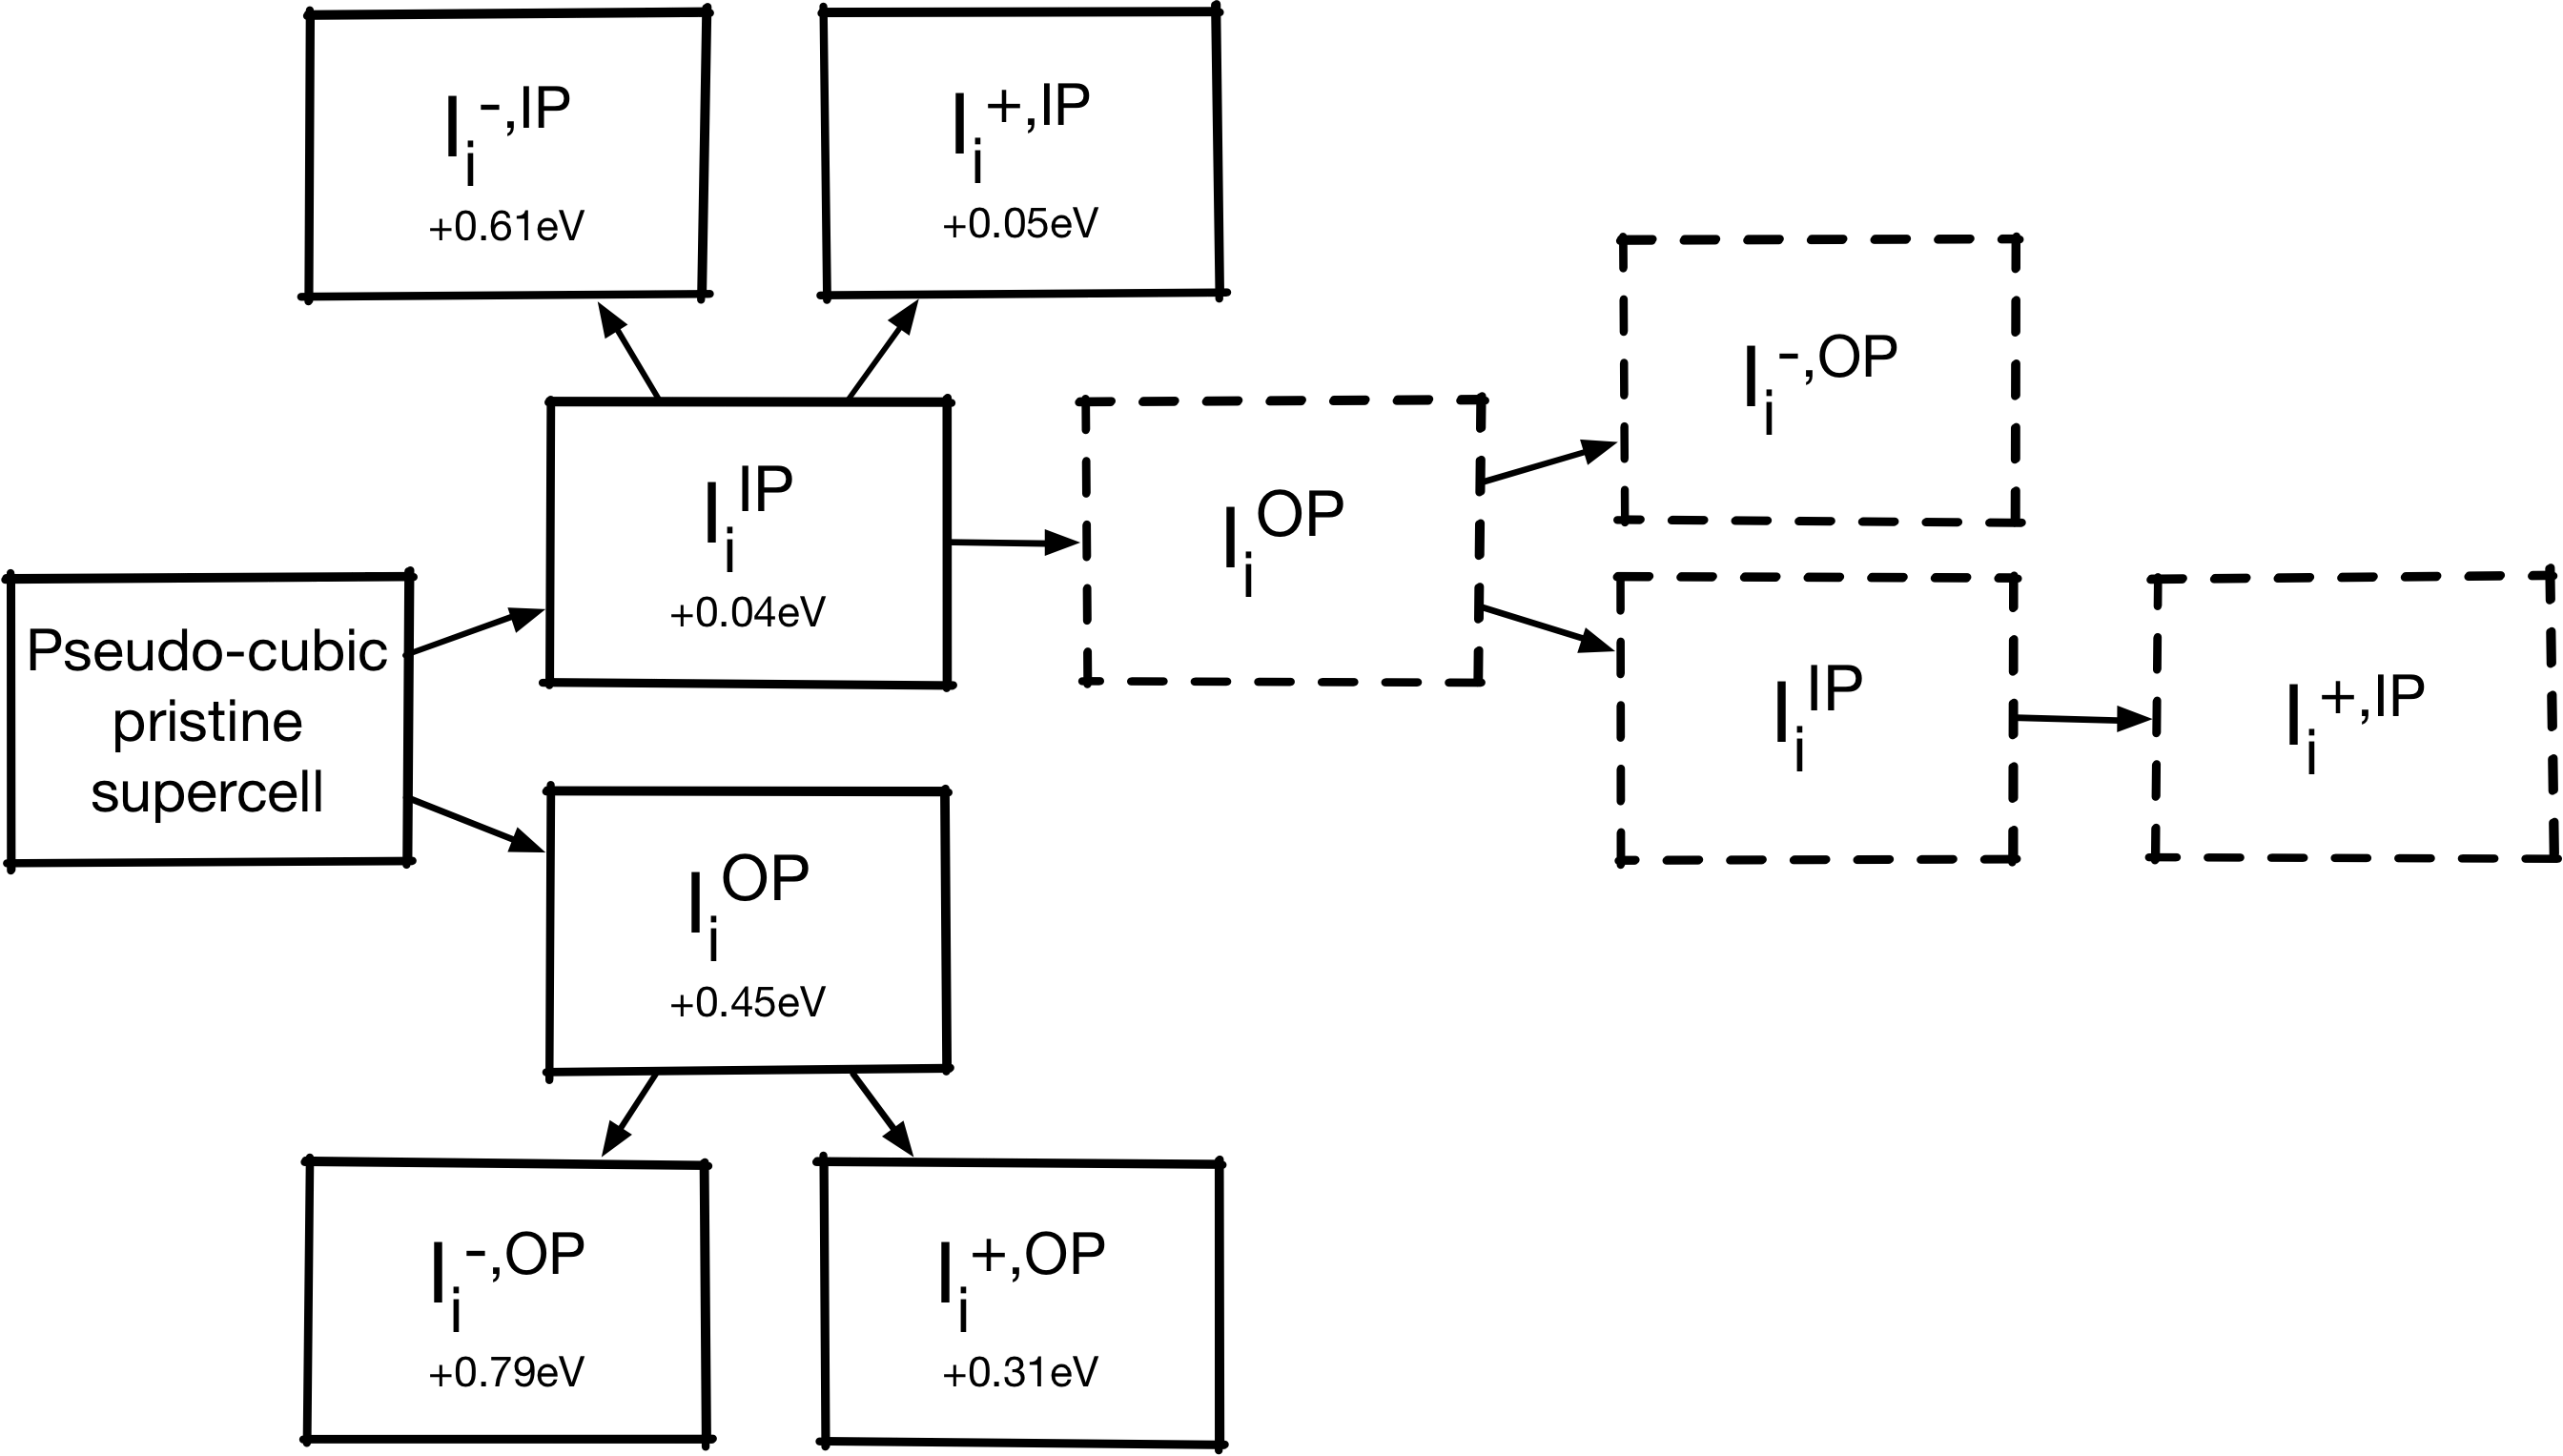
\includegraphics[width=0.7\columnwidth]{figures/ch6/relaxation_workflow.png}
  \caption[Atomic relaxation procedure for point defects in MAPI]{Atomic relaxation procedure for point defects in MAPI. IP indicates that the defect is lying in the $ab$-plane, and OP indicates that the defect is lying along the $c$-axis. The lowest energy structures are in a dash-line box. The hybrid halide perovskite structure has a number of local minima and multiple relaxations were required to break symmetry and reach a global minimum. For the higher energy defect structures the energy above the global minimum for that charge state is given.}
\label{relaxation_workflow}
\end{figure}

In this section the defect geometries of the neutral, negative and positive charge states of the iodine interstitial are given. So that no preference was given to a particular combination of octahedral tilts the starting point for atomic relaxation was MAPI in the pseudo-cubic phase. Upon adding an iodine interstitial the structure was found to have a number of local minima and multiple relaxations between charge states were required to reach a global minimum. To calculate the collective atomic displacement ($\Delta Q$) between charge states accurately the starting point for relaxation of the charged states must be the neutral charge state geometry. The atomic relaxation procedure is outlined in Figure \ref{relaxation_workflow}.

The neutral iodine interstitial $\mathrm{I}_\mathrm{i}$ relaxes to two defect geometries which differ by only \SI{0.04}{\electronvolt} in energy. The lowest energy structure contains a $\mathrm{I}_2^-$ split interstitial that lies out-of-plane (along the $c$-axis) with bond length \SI{3.19}{\angstrom}. This defect is denoted $\mathrm{I}_\mathrm{i}^{\textrm{OP}}$. The higher energy structure contains a $\mathrm{I}_2^-$ split interstitial that lies in the $ab$-plane with bond length \SI{3.24}{\angstrom}. This is denoted $\mathrm{I}_\mathrm{i}^{\textrm{IP}}$. The negative iodine interstitial 
$\mathrm{I}_\mathrm{i}^-$ relaxes to an out-of-plane position along the $c$-axis. $\mathrm{I}_\mathrm{i}^-$ forms a split interstitial around a lattice iodine site with two independently coordinated iodine ions symmetrically bridging two lead atoms. The I--I distance is \SI{3.82}{\angstrom}. As $\mathrm{I}_\mathrm{i}^-$ lies out-of-plane, we expect potential charge trapping processes to occur between $\mathrm{I}_\mathrm{i}^-$ and $\mathrm{I}_\mathrm{i}^{\textrm{OP}}$. The positive interstitial forms an in-plane trimer structure with bond lengths \SI{2.89}{\angstrom} and \SI{2.95}{\angstrom}. As $\mathrm{I}_\mathrm{i}^+$ lies in-plane, we expect potential charge trapping processes to occur between $\mathrm{I}_\mathrm{i}^+$ and $\mathrm{I}_\mathrm{i}^{\textrm{IP}}$.
Table \ref{compare_geoms} contains a summary of the defect geometries and a comparison to values in the literature.

\begin{table}[h!]\centering
\begin{tabular}{llllllll}\toprule
\phantom{abcd}&\multicolumn{2}{c}{This work} &\phantom{a} &\multicolumn{2}{c}{Meggiolaro et al., Ref. \cite{Meggiolaro2018}}&\phantom{a} & Du, Ref. \cite{Du2015} \\
\cline{2-3} \cline{5-6} \cline{8-8}
& orientation & I--I bond length && orientation & I--I bond length  && orientation \\  
\midrule
$\mathrm{I}_\mathrm{i}^-$ &  out-of-plane & 3.82  &&  out-of-plane & 3.89 && in-plane \\
$\mathrm{I}_\mathrm{i}^+$ & in-plane & 2.89/2.95 && in-plane & 2.95 average && in-plane \\
$\mathrm{I}_\mathrm{i}^\mathrm{OP}$ & out-of-plane & 3.19 && out-of-plane & 3.24 && - \\
$\mathrm{I}_\mathrm{i}^\mathrm{IP}$ & in-plane & 3.24 && in-plane & 3.88 && - \\
\end{tabular} 
\caption[Defect orientation and bond length of the $\mathrm{I}_\mathrm{i}^+$, $\mathrm{I}_\mathrm{i}^-$, $\mathrm{I}_\mathrm{i}^\mathrm{IP}$ and $\mathrm{I}_\mathrm{i}^\mathrm{OP}$ defects in MAPI]{\label{compare_geoms}Defect orientation and bond length of the $\mathrm{I}_\mathrm{i}^+$,$\mathrm{I}_\mathrm{i}^-$,$\mathrm{I}_\mathrm{i}^\mathrm{IP}$ and $\mathrm{I}_\mathrm{i}^\mathrm{OP}$ defects in MAPI, with a comparison to computational results in the literature. The bond lengths are given in $\AA$.}
\end{table}

\begin{figure}[h!]
\centering
  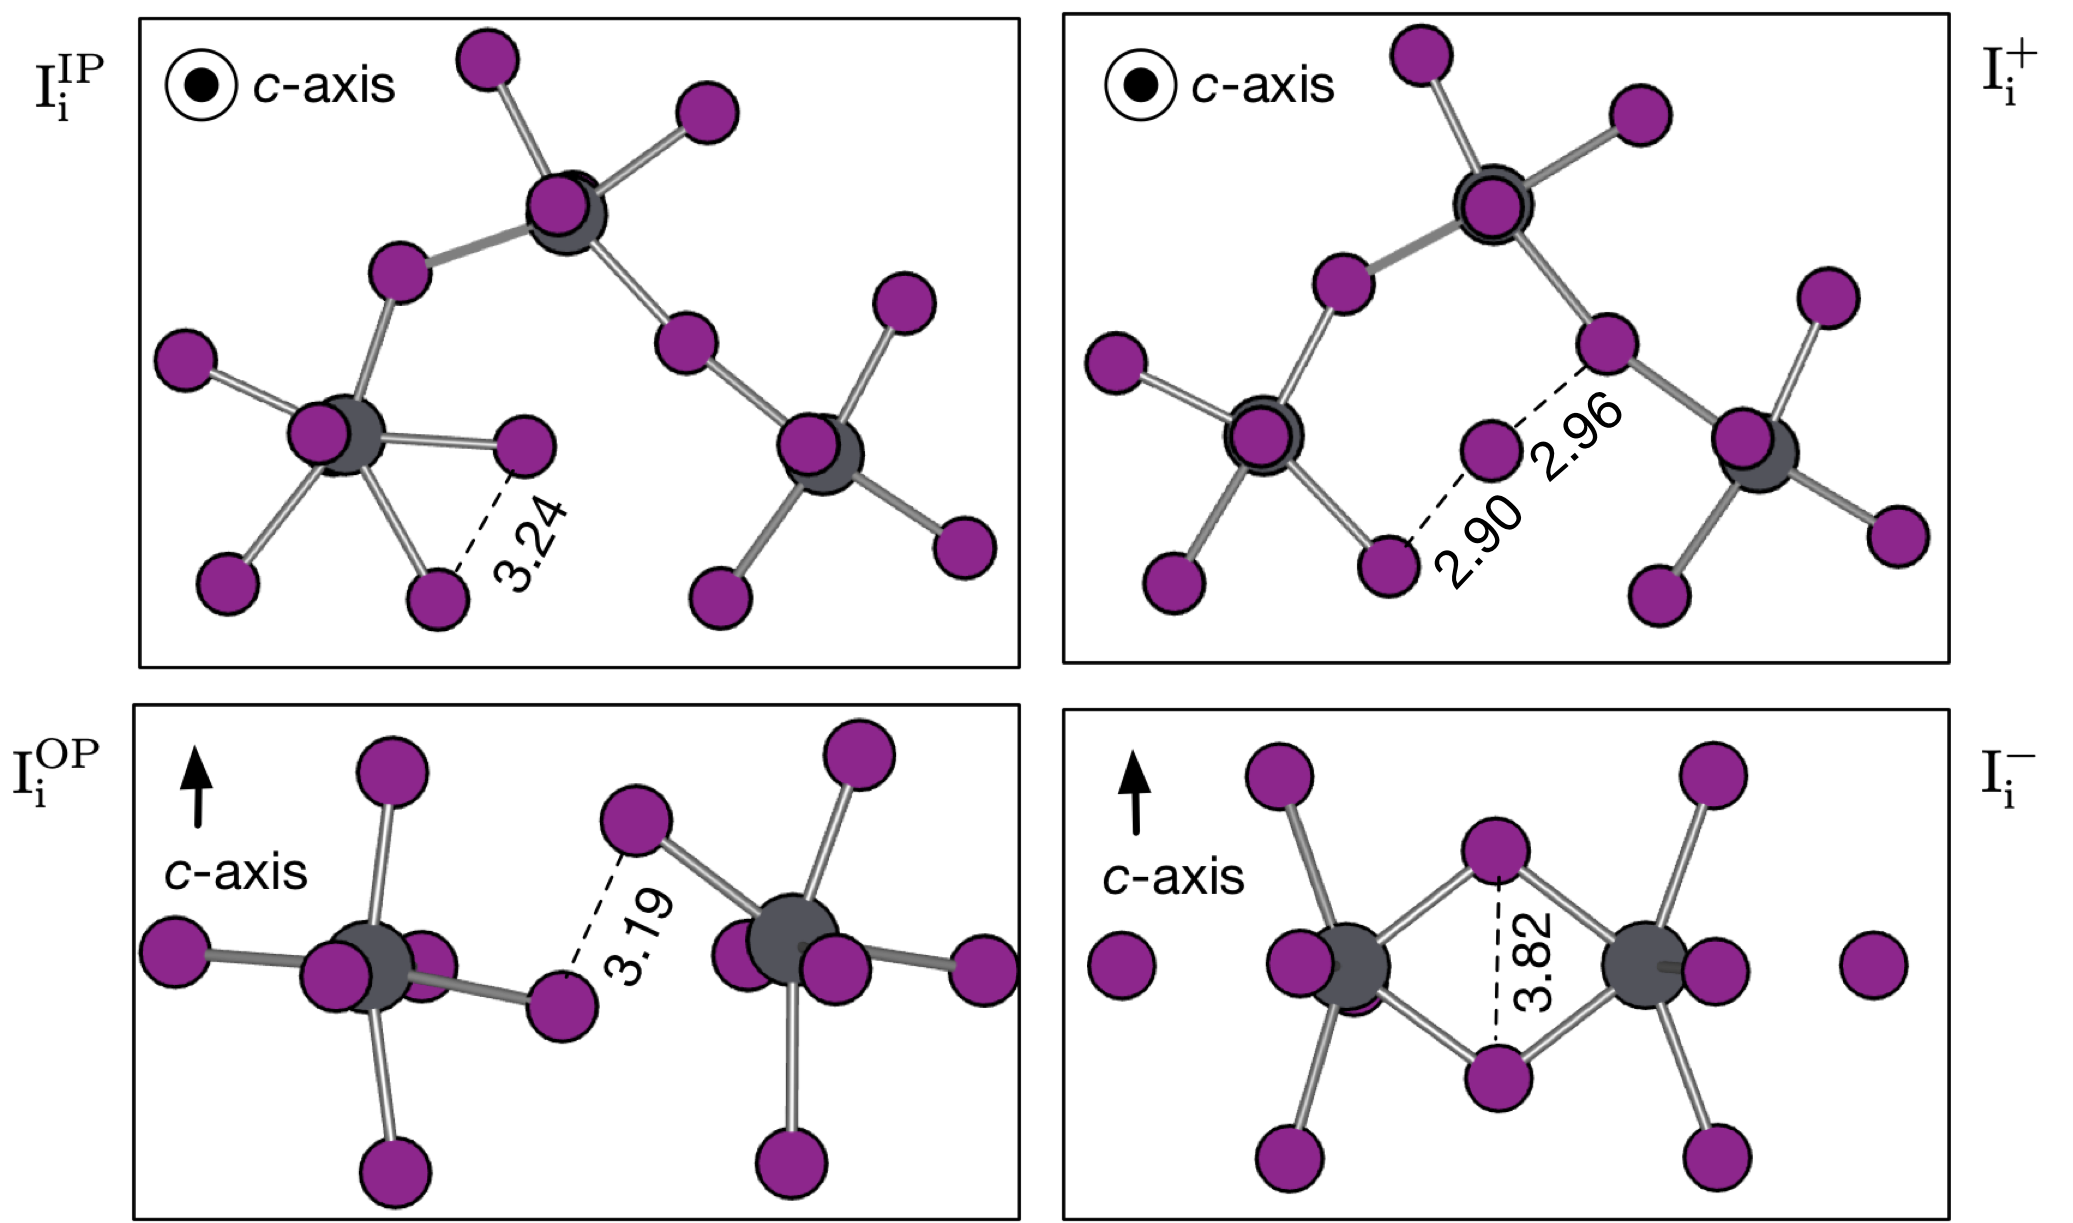
\includegraphics[width=1.0\columnwidth]{figures/ch6/defect_geometries.png}
  \caption[Defect geometries of the $\mathrm{I}_\mathrm{i}^+$,$\mathrm{I}_\mathrm{i}^-$,$\mathrm{I}_\mathrm{i}^\mathrm{IP}$ and $\mathrm{I}_\mathrm{i}^\mathrm{OP}$ defects in MAPI]{Defect geometries of the $\mathrm{I}_\mathrm{i}^+$,$\mathrm{I}_\mathrm{i}^-$,$\mathrm{I}_\mathrm{i}^\mathrm{IP}$ and $\mathrm{I}_\mathrm{i}^\mathrm{OP}$ defects in MAPI. IP indicates that the defect is lying in the $ab$-plane. OP indicates that the defect is lying along the $c$-axis. All distances are measured in $\AA$.}
\label{relaxation_workflow}
\end{figure}

Iodine ions are well known to form polyiodide chains with bond lengths that are sensitive to the charge on each iodine.
The I--I bond length in solid orthorhombic crystalline iodine is \SI{2.67}{\angstrom}, which lengthens to \SI{3.23}{\angstrom} upon formation of $\mathrm{I}_2^-$.\autocite{Chen1985} The bonding lengths reported in this work are within \SI{0.05}{\angstrom} of this value.
The asymmetric bonding of the trimer structure is a typical feature of the tri-iodide group $I_3^-$. For example the tri-iodide group in \ce{CsI_3} has interbond distances of \SI{2.82}{\angstrom} and \SI{3.10}{\angstrom}, with the longer bond possessing the majority of the additional charge.\autocite{Finney1973}
% discuss inequivalent iodine
% include displacement vectors, perhaps in appendix (mention script)

\subsection{Charge localisation} \label{ss:chglocal}
The neutral iodine interstitial forms a spin-radical with a self-trapped hole, as demonstrated in the spin-density plot, Figure \ref{spin_localisation}b.
The hole induces the formation of a bond between two iodine ions, producing a molecular dimer called a H-centre (Figure \ref{spin_localisation}a). The formation of a H-centre is a well-established process, and has been studied in metal halide crystals since the 1950s.\autocite{Castner1957} In Figure \ref{spin_localisation}b we see that there is some charge delocalisation across the outer halogens, as has been found for H-centres in the alkali halides.\autocite{Shluger1995}
Whereas in the previous chapter we considered a large polaron, in this chapter we are studying a small polaron formed by the self trapped hole.

\begin{figure}[h!]   %includes H-centre schematic
\centering
  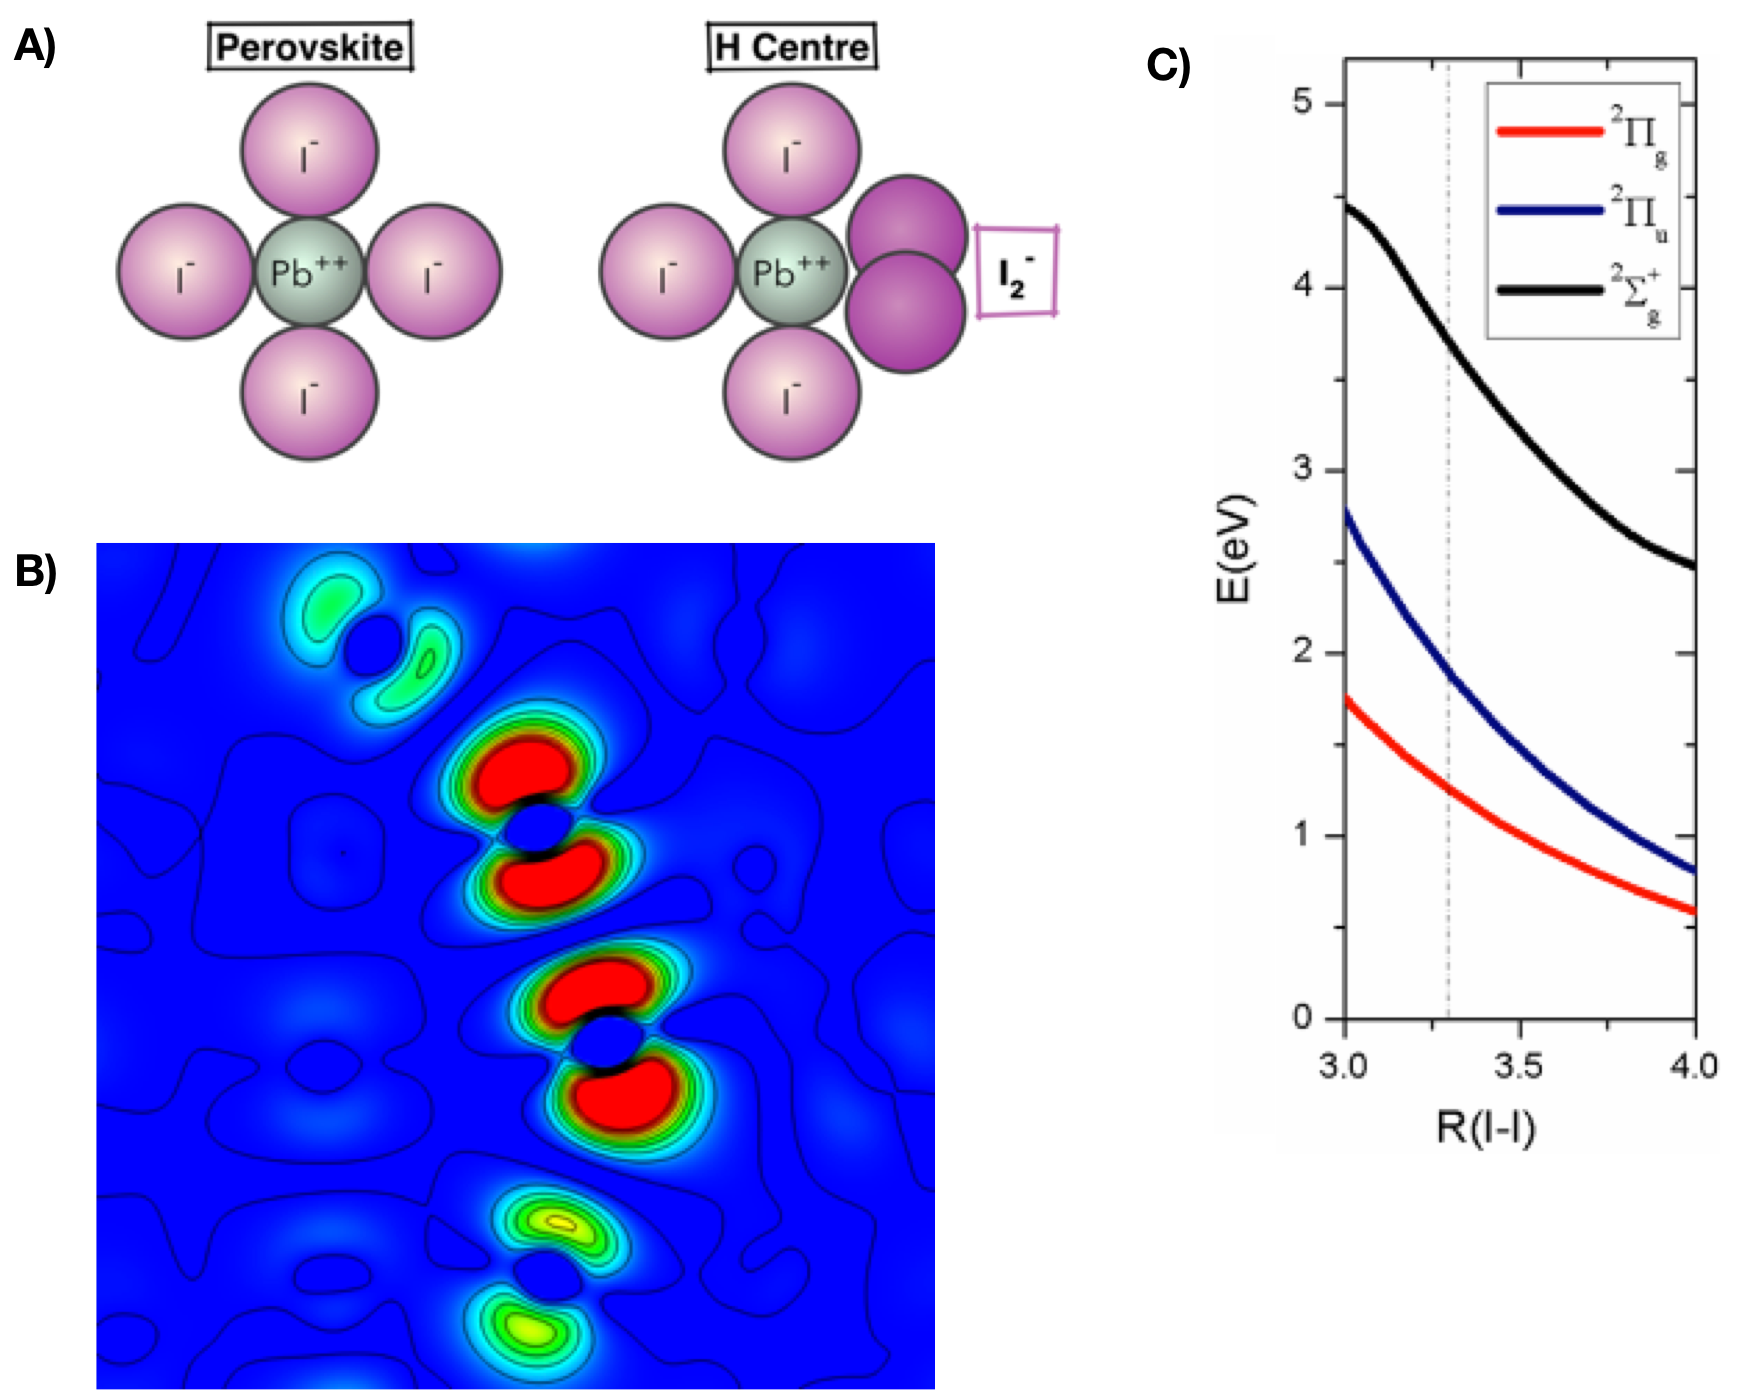
\includegraphics[width=0.9\columnwidth]{figures/ch6/spin_localisation.png}
  \caption[Spin localisation and optical excitation at the H-centre defect in MAPI]{A) Change in local equatorial environment around Pb in a lead halide perovskite upon formation of a H-centre defect. The H-centre is formed from a lattice iodide and interstitial iodide. The I--I interatomic spacing of ca. \SI{4.5}{\angstrom} in the perfect lattice decreases to a bond length of \SI{3.2}{\angstrom} upon dimer formation. Figure adapted with permission from an original prepared by Aron Walsh. B)  The difference between the density of the two spin channels in a spin-polarised calculation is plotted to show spin localisation around the H-centre defect in MAPI. C) Optical excitation energies as a function of dimer bond length for the iodine dimer in MAPI. The bond length is given in $\AA$.}
\label{spin_localisation}
\end{figure}
%include updated TDDFT results

The H-centre is a `molecule-in-a-crystal' defect where the host weakly perturbs the $I_2^-$ molecular ion.
This allows us to consider the optically excited states using a dielectric embedding approach.
A collaborator, Rachel Crespo-Otero, has computed the optically excited states of the H-centre defect as a function of bond lengths using time-dependent DFT including relativistic effects (Figure \ref{spin_localisation}c).\autocite{Whalley2017b} 
%For a bond lengths found in the MAPI host (\SI{3.19}{\angstrom}), the three lowest excited states occur at \SI{}{\electronvolt} (symmetry-allowed), \SI{}{\electronvolt} (forbidden), and \SI{}{\electronvolt} (symmetry-allowed). Two optically allowed transitions fall in the visible−ultraviolet range, and a sub-band gap absorption band at ca. \SI{}{\electronvolts} should be observable in long-wavelength absorption measurements if present in sufficient concentration.
For a bond length of \SI{3.28}{\angstrom}, the three lowest excited states occur at \SI{1.26}{\electronvolt} (symmetry-allowed), \SI{1.90}{\electronvolt} (forbidden), and \SI{3.70}{\electronvolt} (symmetry-allowed). Two optically allowed transitions fall in the visible−ultraviolet range, and a sub-band gap absorption band at ca. \SI{1.3}{\electronvolts} should be observable in long-wavelength absorption measurements if present in sufficient concentration.

\subsection{Defect formation energies} \label{ss:dfe}

The formation energy of a defect in charge state $q$ is given by
\begin{equation} \label{eqn_formation_energy}
E_\mathrm{f}(q) = E_\mathrm{d}(q) - E_\mathrm{b} - \sum_i \mu_i n_i + q(\epsilon_\mathrm{VBM}+E_\mathrm{F}) + E_\mathrm{corr}.
\end{equation}
The total energy of the supercell $E_\mathrm{d}(q)$, the total energy of the pristine lattice $E_\mathrm{b}$ and the iodine chemical potential $\mu_i$ were calculated DFT as outlined in the methods section.
The defect correction $E_\mathrm{corr}$ consists of two terms - the image charge correction for charged defects and a `tilting' correction that is specific to pseudo-cubic perovskites.
The image charge correction is \SI{-0.057}{eV}. The static dielectric constant of MAPI is large ($\bar{\epsilon_0}=22.67$)\autocite{Brivio2013} and so the lattice can effectively screen charged defects, in addition the point defects in this study have a maximum charge of one and the supercell is relatively large (193 atoms). These factors lead to a small image charge correction.

\begin{figure}[h!]   
\centering
  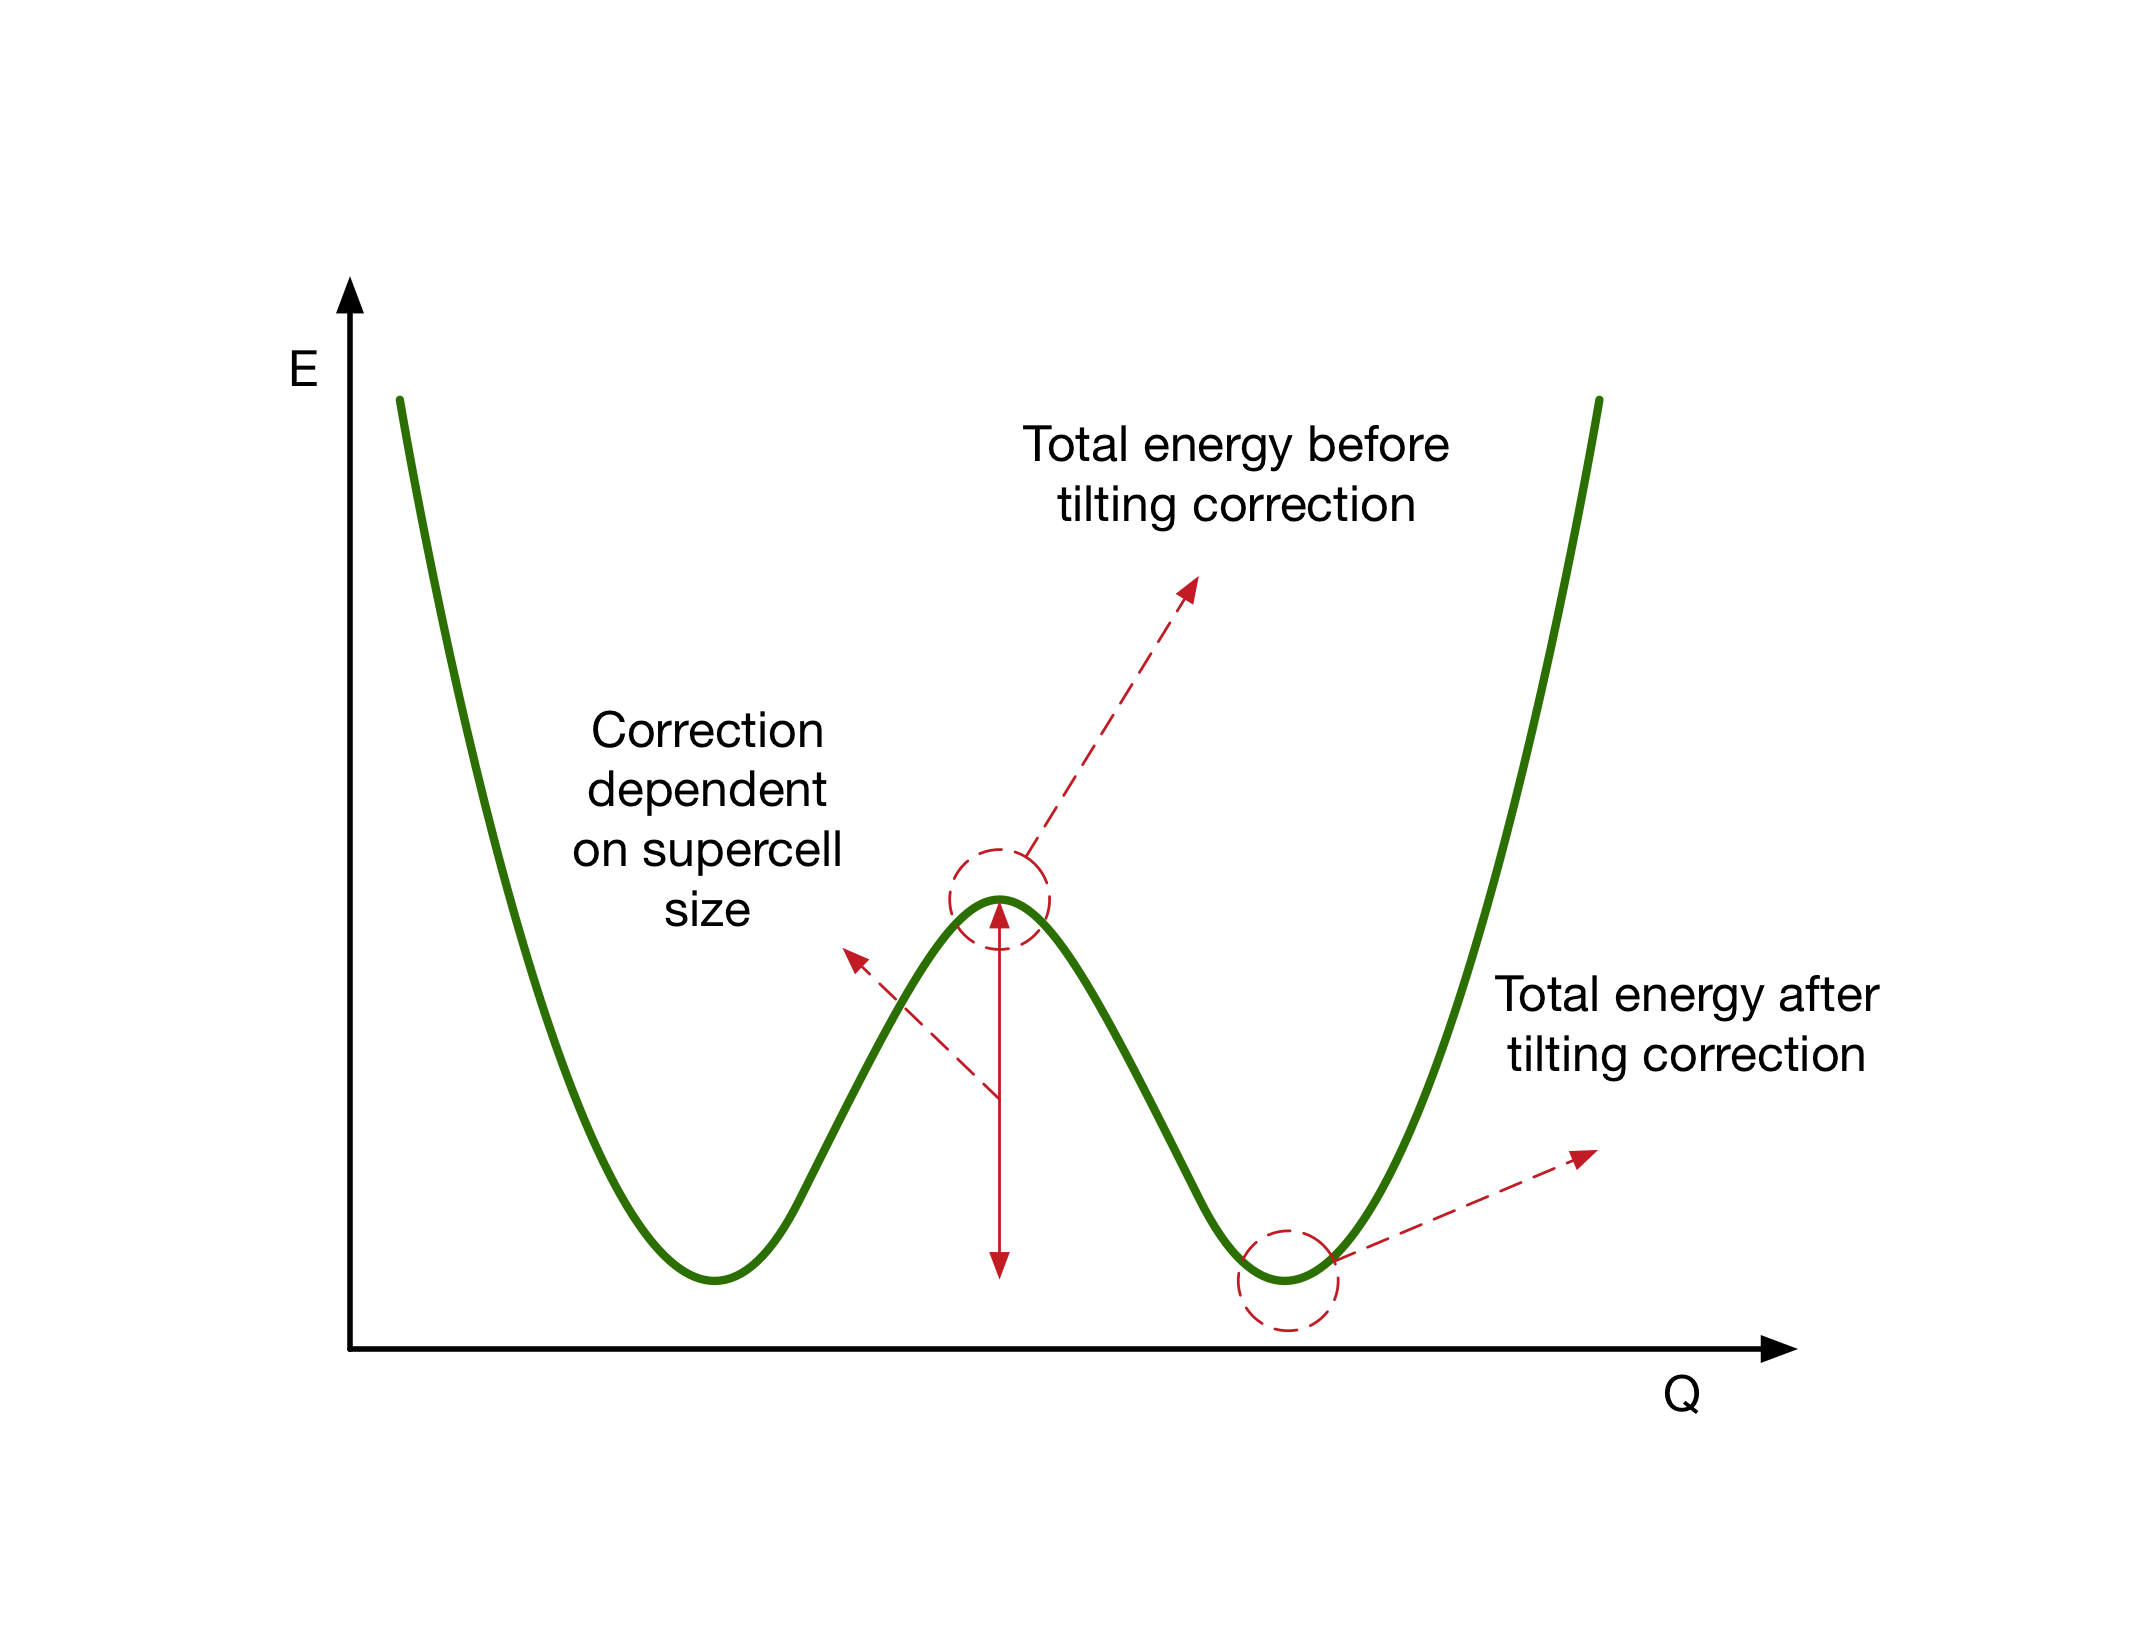
\includegraphics[width=0.8\columnwidth]{figures/ch6/tilting_correction.png}
  \caption[Tilting correction for the pseudo-cubic perovskite lattice]{A schematic of the tilting correction used in this work. The green line is the double well potential energy surface that is typical of pseudo-cubic perovskite structures. This correction to defect formation energy is only needed when using the high-symmetry pseudo-cubic perovskite phase to calculate the pristine bulk energy.}
\label{tilting_correction}
\end{figure}

\begin{table}[h!]\centering
\begin{tabular}{lll}\toprule
supercell expansion&\# atoms&tilting correction (meV) \\ 
\midrule
$2\,\times\,2\,\times\,2$ & 96 & 37 (calculated) \\
$4\,\times\,4\,\times\,4$ & 768 & 270 (calculated) \\
$2\sqrt2\times2\sqrt2\times2$ & 192 & 74 (predicted) \\
\bottomrule
\end{tabular} 
\caption[Tilting corrections for supercell expansions of the pseudo-cubic perovskite lattice]{\label{modemaptable} Tilting corrections for supercell expansions of the pseudo-cubic perovskite lattice. The 768-atom supercell is eight times larger than the 96-atom supercell, so we expect the tilting correction to be eight times larger. It is calculated to be 7.5 times larger. The tilting correction for the 192-atom expansion, which cannot be calculated directly, is twice as large as the correction for the 96-atom supercell. }
\end{table}

The tilting correction is a new correction introduced in this work and is particular to the pseudo-cubic perovskites. All of the defect formation energies are referenced to a pristine lattice energy. The geometry of the pristine lattice in the pseudo-cubic phase corresponds to a time average and is not the minimum energy structure (Figure \ref{tilting_correction}). To calculate the minimum energy geometry the pseudo-cubic structure can be distorted along the soft mode at the $R$-point in $q$-space. This `modemapping' procedure\autocite{Skelton2016a} is not compatible with the supercell expansion used for the 197-atom supercell, but the correction energy can be inferred from modemapping other supercell expansions (Table \ref{modemaptable}).

The charge transition diagram is given in Figure \ref{charge_transition_diagram}. 
As is found in the previous literature\autocite{Du2015,Meggiolaro2018} there is negative-U behaviour, where the (+/0) transition level is higher in energy than the (0/-) transition. This indicates that on electron trapping there is a strong structural relaxation around the defect. The neutral charge state in both orientations is thermodynamically unstable across the Fermi energy range and is formed after photo-excitation. As in Reference \cite{Meggiolaro2018} the out-of-plane neutral charge state is lower in energy than the in-plane neutral charge state.

\begin{figure}[h!]   
\centering
  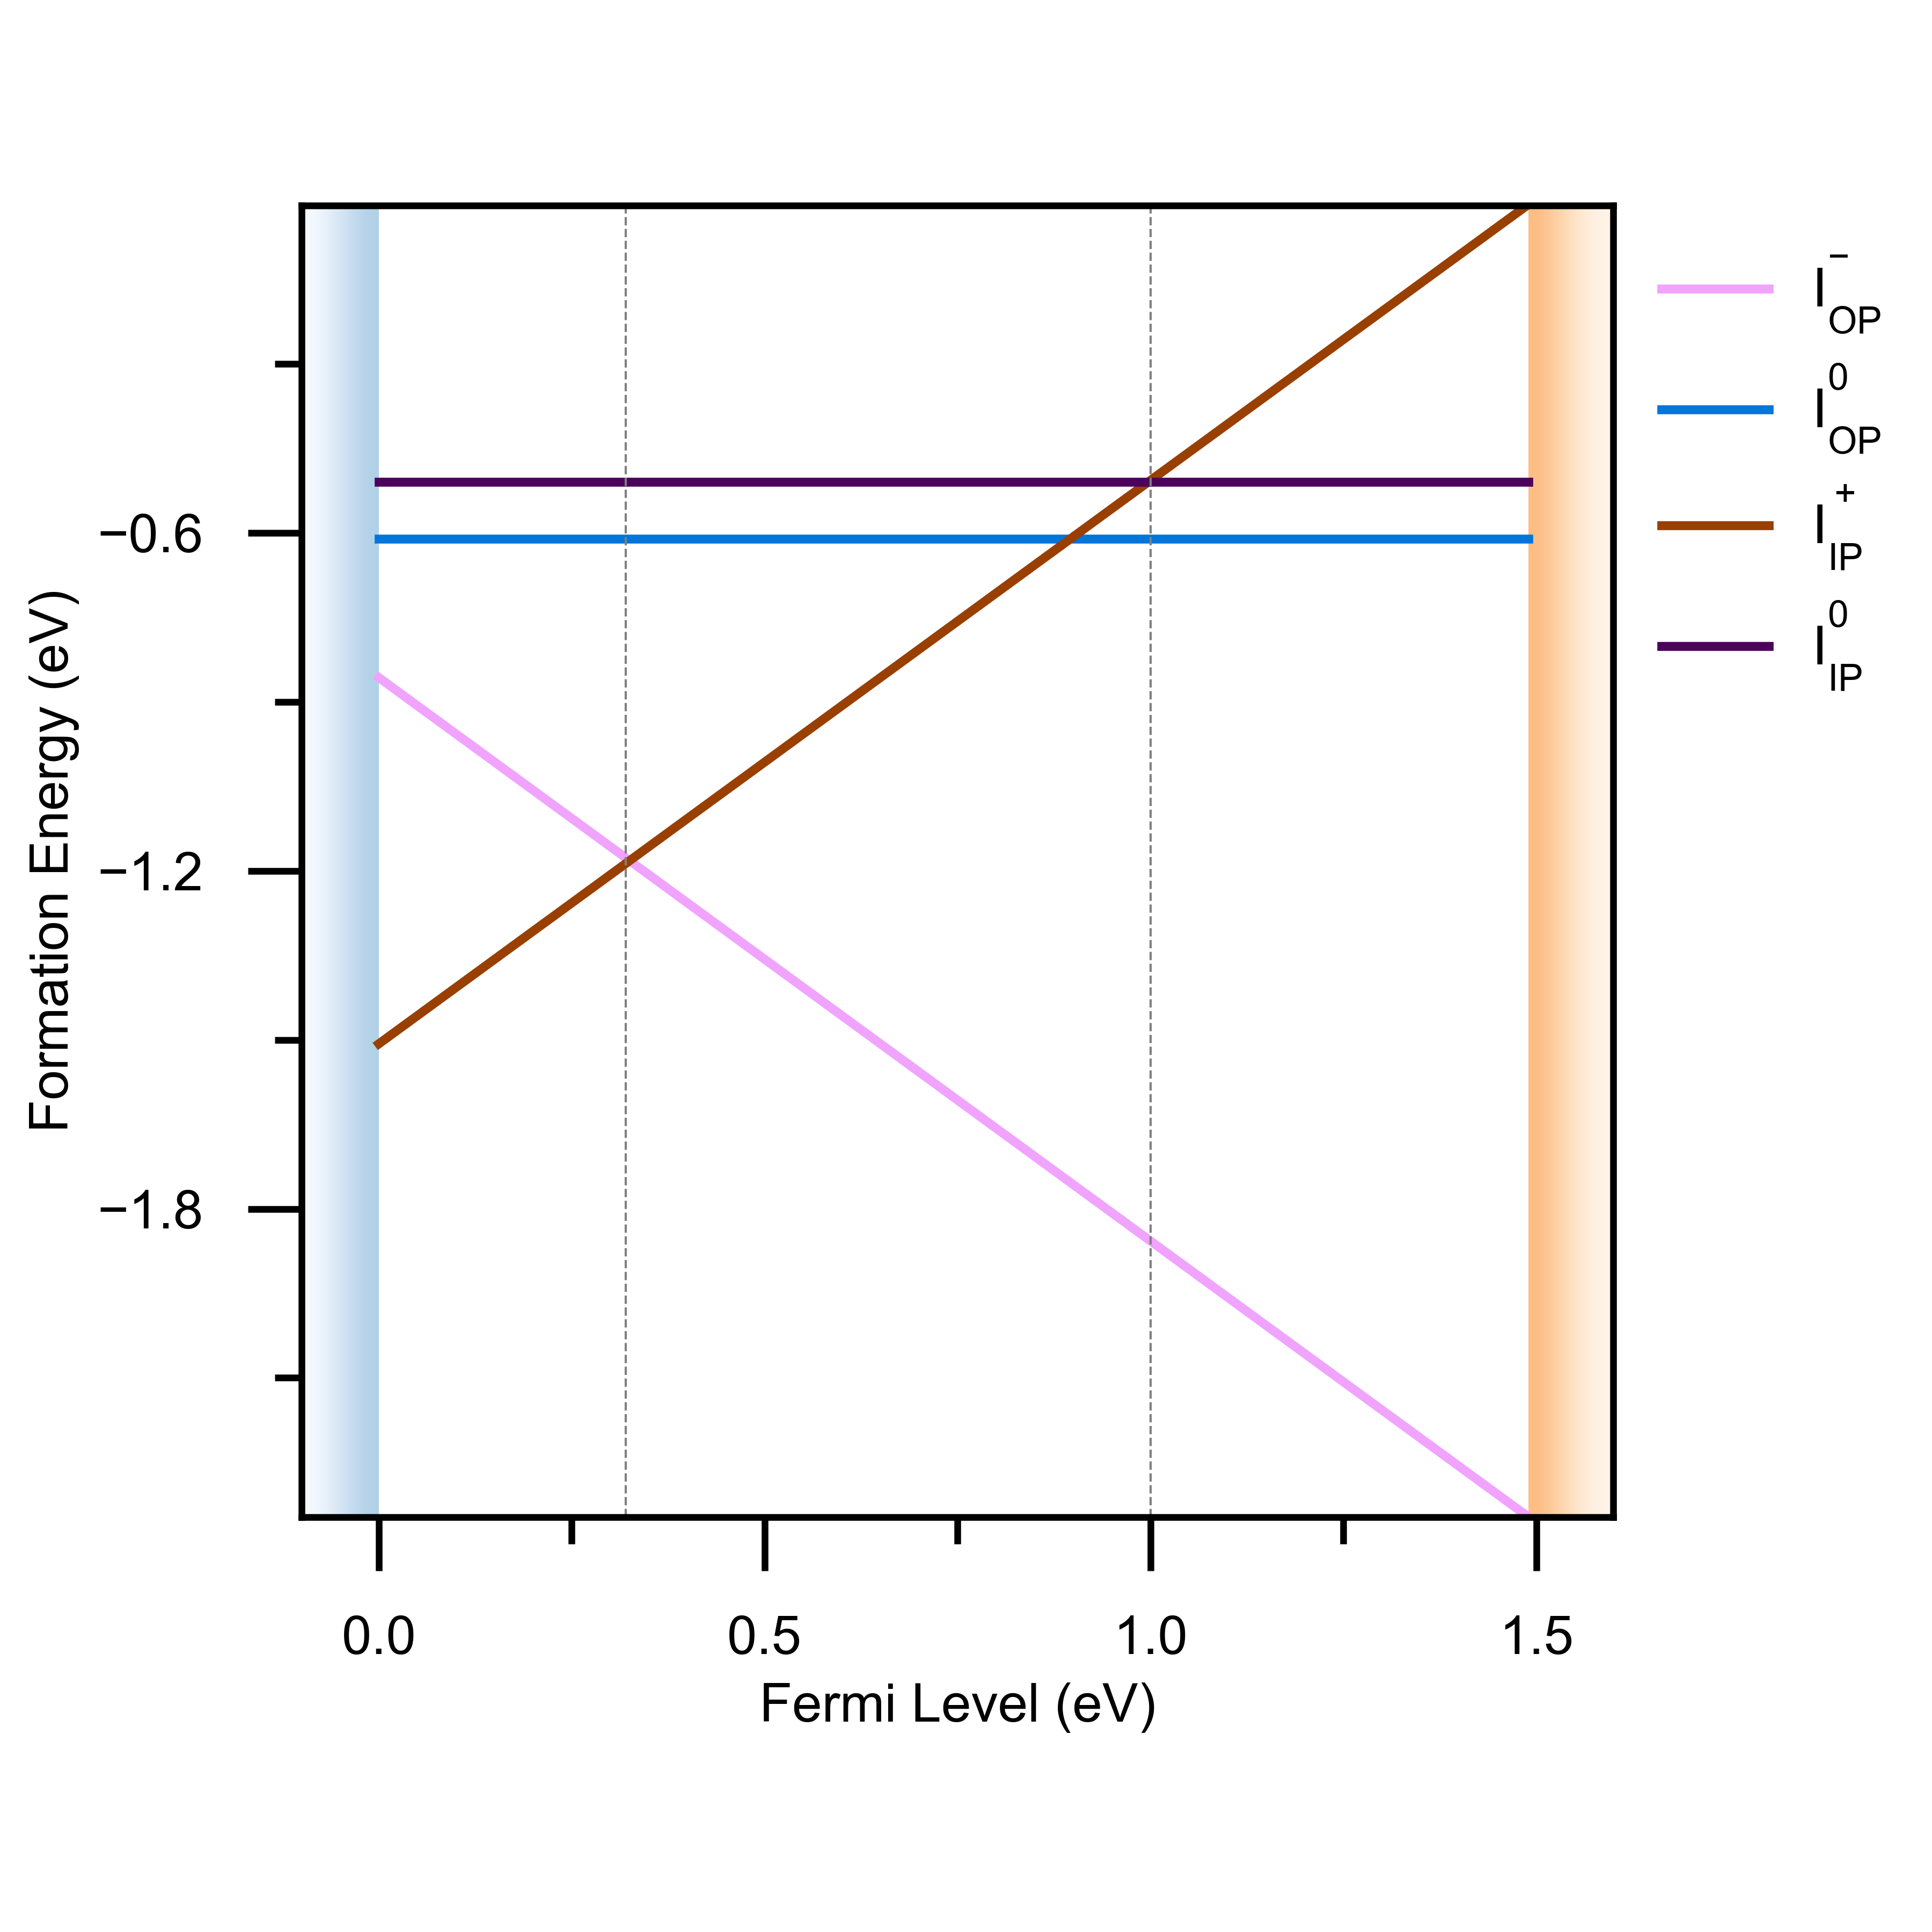
\includegraphics[width=0.7\columnwidth]{figures/ch6/charge_transition_HSE.png}
  \caption[Charge transition diagram for the iodine interstitial defect in MAPI]{Charge transition diagram for the iodine interstitial defect in MAPI, calculated using the hybrid HSE06 funtional with spin-orbit coupling. IP indicates that the defect is lying in the $ab$-plane and OP indicates that the defect is lying along the $c$-axis.}
\label{charge_transition_diagram}
\end{figure}
% need to update defect notation!

There is one active charge trapping level in the bandgap, corresponding to electron trapping at $\mathrm{I}_\mathrm{i}^+$.  The (+/-) level corresponds to a two-electron transition and we assume that the cross section for this process is negligible. This result is in contrast to previous reports which find that there are two active charge trapping levels in the bandgap -- electron trapping at $\mathrm{I}_\mathrm{i}^+$ and hole trapping at $\mathrm{I}_\mathrm{i}^-$.
The charge transition diagram generated using the intermediate higher energy structures (Figure \ref{relaxation_workflow}) reproduces the results in the literature. This highlights how sensitive the defect energetics are to defect geometry. The charge transition diagram for the intermediate higher-energy defect structures is given in Appendix \ref{app:7-chargetransition}.

The final thing to note is that the defect formation energies are negative across the Fermi level range. This is unphysical, as for a thermodynamically stable material it costs lattice energy to create a point defect. The problem arises from the simple approximation used for the chemical potential of iodine, which considers bulk iodine only and no other competing phases such as \ce{PbI2}. As a result, the chemical potential used in this defect calculation provides an upper bound. Consideration of other secondary phases would produce a lower chemical potential and increase the defect formation energy for all charge states. 
%comment on fermi level pinning

\subsection{Configuration coordinate diagram} \label{ch6:ccd}

Charge trapping between the neutral and negative charge states of the iodine interstitial can be described using a configuration coordinate diagram (Figure \ref{configuration_coordinate}), which gives the total system energy as a function of a single mode $Q$.\autocite{Alkauskas2016} 
The model assumes that the electronic states of the defect interact with only one phonon mode of the lattice, and that
the minimum of each curve corresponds to the equilibrium position of the ions and the electronic ground state. 
To model electron trapping at the neutral charge state, the excited state of the system corresponds to the neutral defect with a photo-generated electron in the conduction band and hole in the valence band, and the ground state corresponds to the negatively charged defect with a hole in the valence band.
Hole trapping at the negative charge state is not possible due to the large energetic barrier of ca. \SI{1}{\electronvolt}.

\begin{figure}[h!]   
\centering
  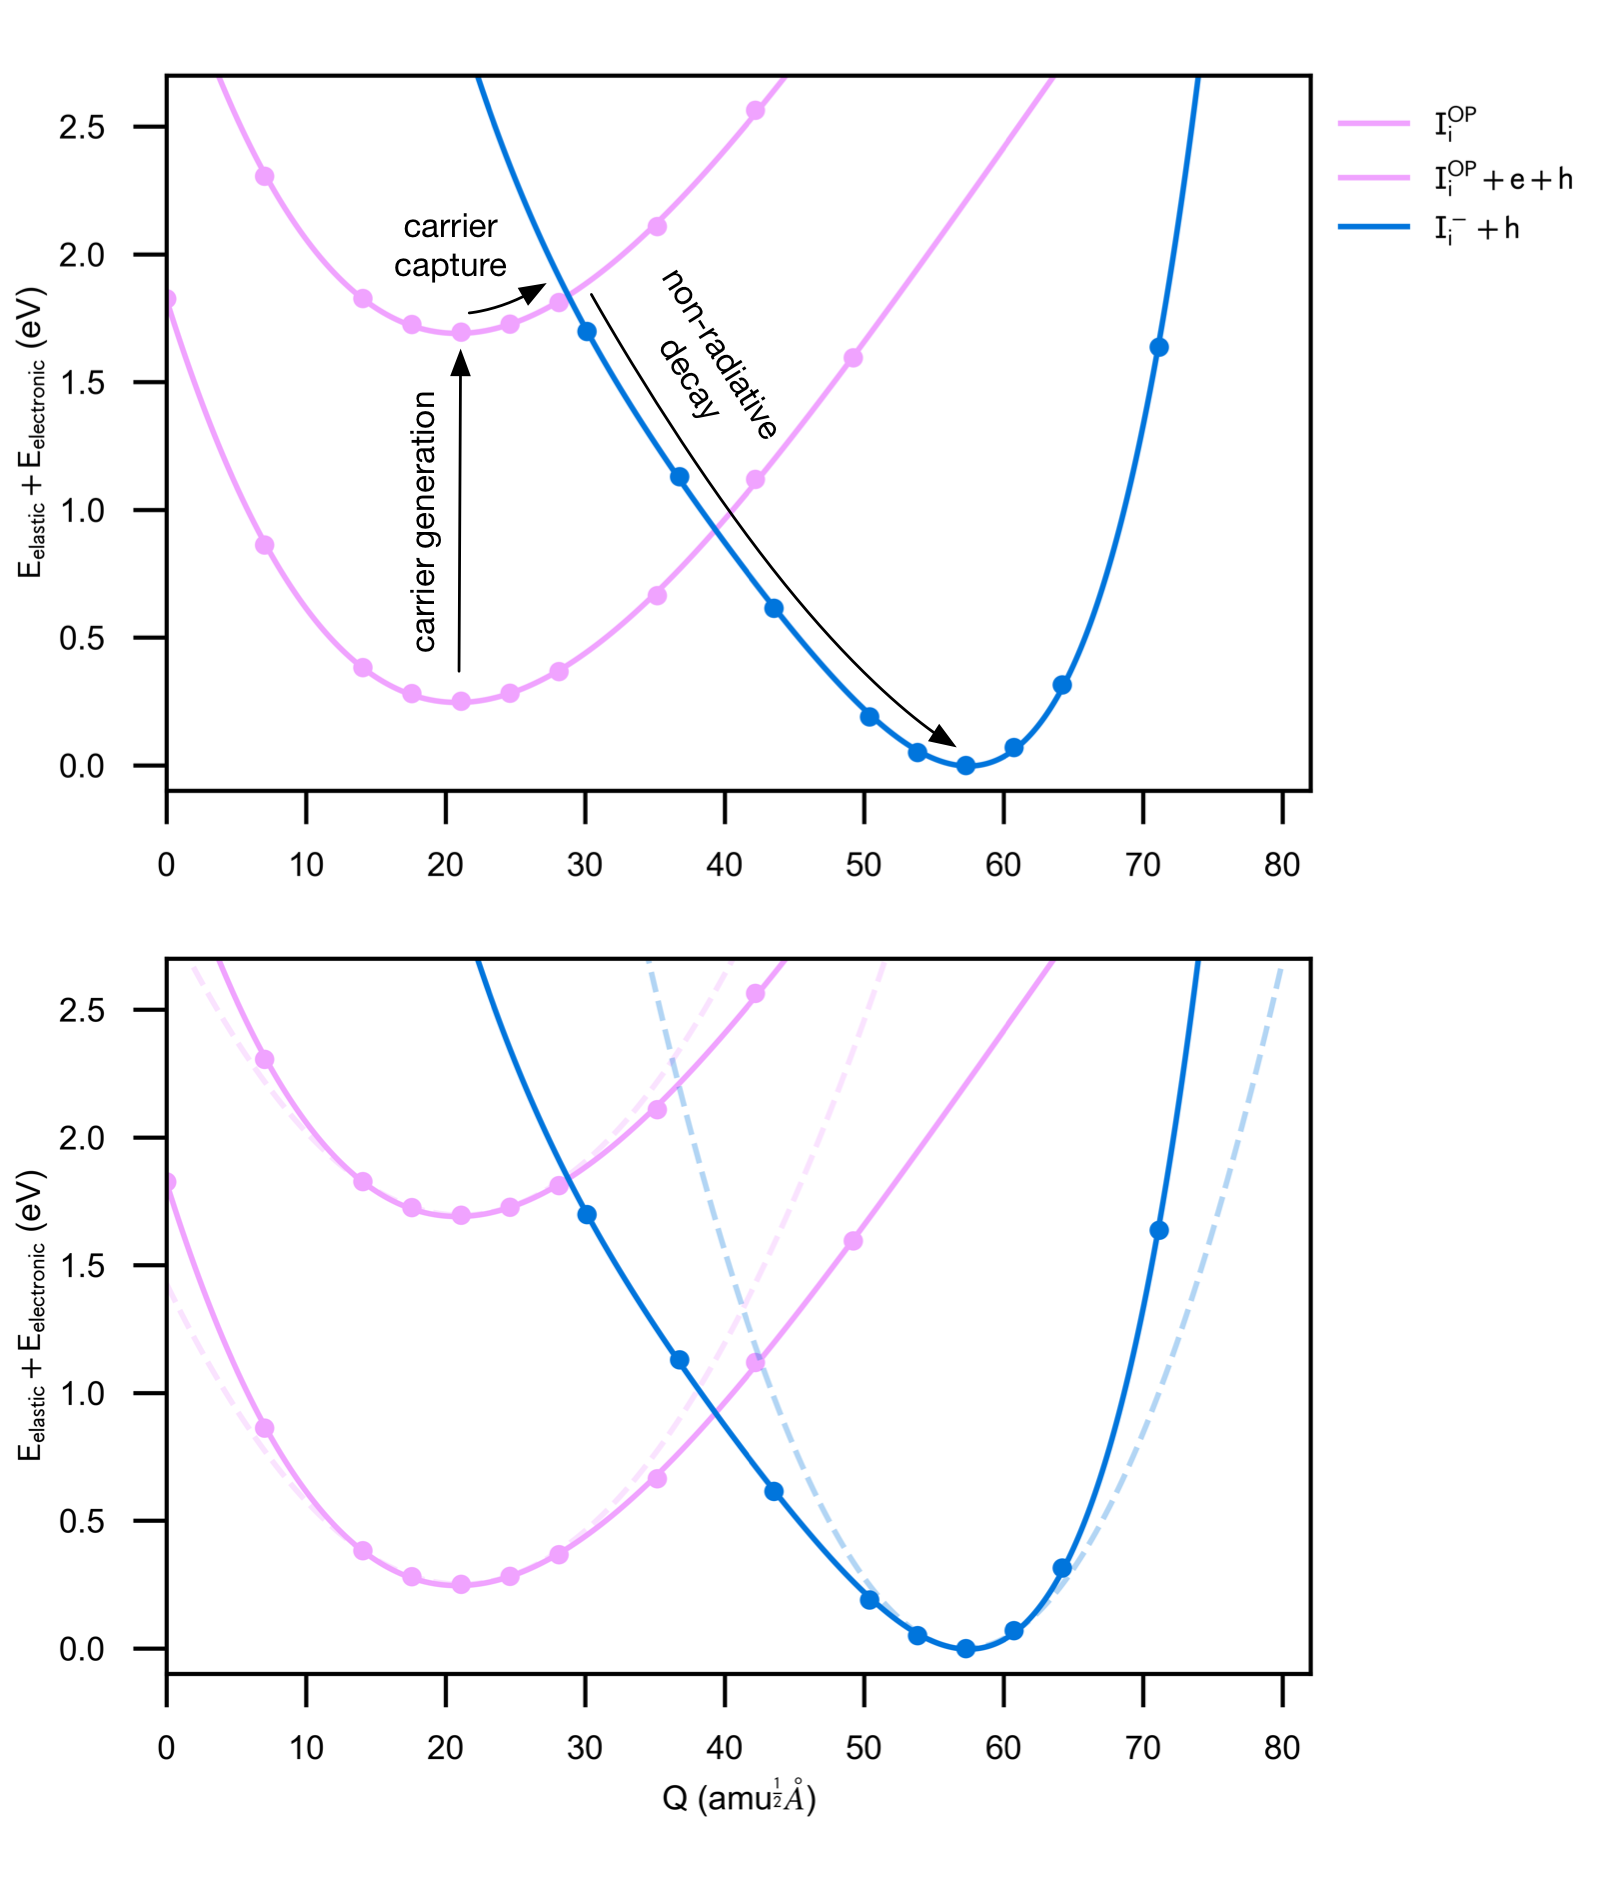
\includegraphics[width=1.0\columnwidth]{figures/ch6/carrier_capture_digram.png}
  \caption[Configuration coordinate diagram describing carrier capture between negative and neutral charge states of the iodine interstitial defect]{(Top) Configuration coordinate diagram describing carrier capture between the negative and neutral charge states of the iodine interstitial defect. The potential energy surfaces are calculated using the hybrid HSE06 functional with spin-orbit coupling. (Bottom) A comparison between the anharmonic and harmonic potential energy surfaces. To model electron trapping at the neutral charge state, the excited state of the system corresponds to the neutral defect with a photo-generated electron in the conduction band and hole in the valence band, and the ground state corresponds to the negatively charged defect with a hole in the valence band. }
\label{configuration_coordinate}
\end{figure}
% talk ahout the difference between the photochemistry and equilibrium thermodynamics


In this work this the configuration coordinate $Q$ is defined as $\sqrt{\sum_i m_i \Del r_i^2}$ ,where the sum is over all inorganic atoms $i$ with mass $m_i$ and a displacement from equilibrium of $\Del r_i$. Summing over all atoms, including those in the organic methylammonium molecule, led to unphysical energies as the linear interpolation does not capture the rotation of the organic cation between charge states. The potential energy surface generated using a summation over all atomic displacements is given in Appendix \ref{app:9-configcoord}.

Lattice relaxation after electron capture leads to a large shift in the equilibrium position ($\Delta Q=$ \SI{46}{\electronvolt\per amu\tothe{1/2}\per\angstrom}).
This is double that found for non-radiative recombination centres in CZTS\autocite{Kim2018} and reflects the strong coupling between the electronic charge state of the defect and the lattice distortion. 
Another parameter commonly used to classify defects by electron-phonon coupling strength is the Huang-Rhys factor $S$ which quantifies the number of phonons emitted during an optical transition. For a harmonic potential energy surface the Huang-Rhys factor is given by 
\begin{equation}
S = \frac{E}{\hbar\omega}.
\end{equation}
The Huang-Rhys factor for lattice relaxation after electron capture at the neutral interstitial is 361.7. This is in the strong coupling limit where $S\gg1$. The large lattice distortion and Huang-Rhys factor suggests that there will be fast non-radiative transitions at the defect site.\autocite{Hayes1985,Hughes1967}

The configuration coordinate diagram for this charge capture process has been previously reported by Meggiolaro et al.,\autocite{Meggiolaro2018} where it was found that electron trapping at the neutral iodine interstitial proceeds with a small geometrical rearrangement. However the structural parameter used was the root mean square displacement (RMSD) of the two iodine ions involved with bonding, which excludes the large relaxation of the surrounding perovskite structure. The same RMSD definition applied to the defect geometries in this work gives a lattice distortion of \SI{0.073}{\angstrom}, which appears close to that given in Figure 2 of Reference \cite{Meggiolaro2018}. By considering only the distortion to the bonding iodine and ignoring the wider structural reorganisation Meggiolaro et al. infer that the rate of radiative recombination will compete with non-radiative recombination. Figure \ref{configuration_coordinate} of this work demonstrates that this is not the case and that the large distortion of the surrounding lattice will prevent radiative electron capture at the defect.

The lower part of Figure \ref{configuration_coordinate} compares the anharmonic potential energy surface (PES) to the harmonic PES. The curvature of the harmonic potential energy surface is equal to the difference in energy between the two lowest phonon eigenstates of the anharmonic PES. In Figure \ref{configuration_coordinate} we see that the harmonic PES fits well to the DFT energies either side of the equilibrium structure, as we would expect. The potential energy surfaces of the neutral and negative charge states are extremely soft; for the neutral charge state $\hbar\omega=$\SI{4.7}{meV} (\SI{1.14}{\tera\hertz}) and for the negative charge state $\hbar\omega_0=$\SI{6.6}{meV} (\SI{1.59}{\tera\hertz}). Phonon modes at this energy will lie in the optical band of the MAPI lattice modes and will be occupied at room temperature.

Figure \ref{configuration_coordinate} highlights the importance of using anharmonic potential energy surfaces to describe charge capture at the iodine intersitital in MAPI. The harmonic potential energy surfaces for the excited and ground state intercept at an energy ca. \SI{0.5}{eV} above the excited state equilibrium energy, and this leads to a carrier capture coefficient four orders of magnitude smaller than that calculated for the anharmonic surfaces (values for the coefficient are given in Section \ref{finalsection}).

\subsection{Vibrational properties of MAPI:$\mathbf{I}_\mathbf{i}^\mathbf{-}$}

In the previous section the coupling of the iodine interstitial to a single vibrational mode was considered without reference to harmonic phonon modes of the crystal.
In this section the normal phonon modes of the crystal with a $\mathrm{I}_\mathrm{i}^-$ defect are calculated and analysed.
The normal phonon modes of a crystal containing a defect can be divided into three kinds: lattice modes (optic and acoustic branches), resonant modes, and local modes (Figure \ref{defect_modes_schematic}).\autocite{Stoneham defect defect processes}
The lattice modes are largely unaffected by the defect and are well approximated by the the normal modes of the perfect crystal. They have the same amplitude throughout the crystal, except near the defect where there may be some slight modification. 
Resonant modes have frequencies that lie within the continuum of lattice modes. The motion is strongly enhanced near the defect and diminishes away from the defect.
Finally, local modes have frequencies that lie outside those of the perfect lattice modes. Here the motion is local and dies away to zero far from the defect.

\begin{figure}[h!]   
\centering
  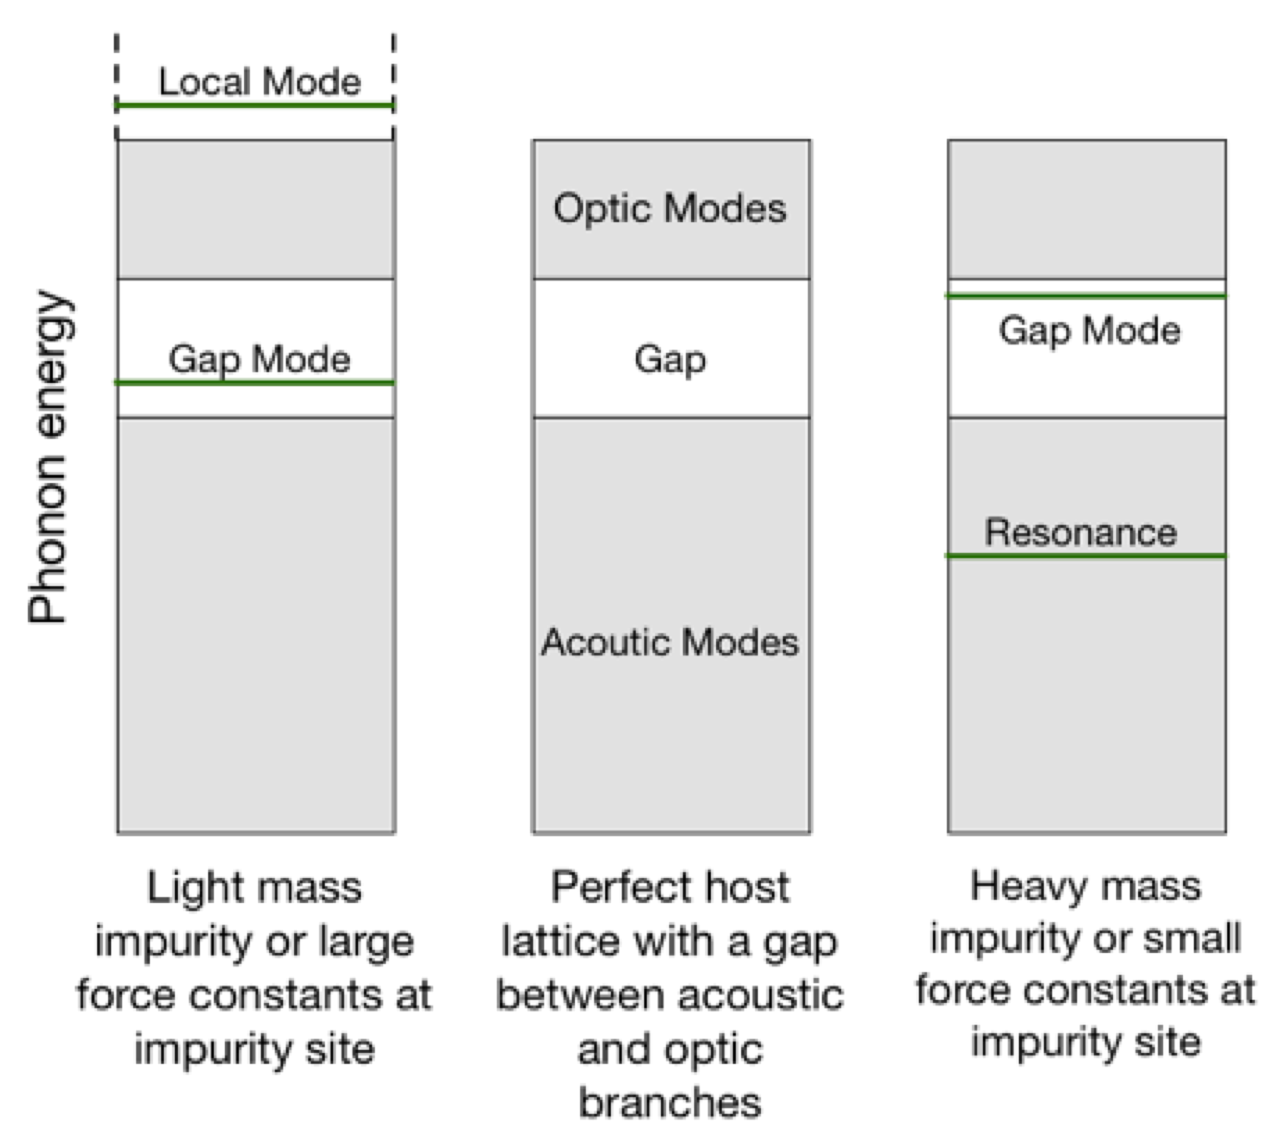
\includegraphics[width=0.6\columnwidth]{figures/ch6/defect_modes_schematic.png}
  \caption[The three kinds of normal phonon modes found in a crystal with a defect]{The three kinds of normal phonon modes found in a crystal with a defect. }
\label{defect_modes_schematic}
\end{figure}  %add the lattice modes, and change gap to local modes, and dont bother about teh different weights of impurity...

The phonon dispersion for the MAPI crystal with an iodine interstitial is given in Figure \ref{defect_dispersion_IPR}b, with the phonon dispersion for the pristing MAPI crystal in Figure \ref{defect_dispersion_IPR}a for comparison.
The group velocity of a phonon mode is given by $\frac{\delta \omega_k}{\delta k}$. It follows that flat bands are associated with localised phonon modes that do not propagage through the crystal. 
When the defect is introduced the translational symmetry of the crystal is broken and the energetically degenerate modes of the pristine crystal become non-degenerate and increasingly localised.


\begin{figure}[h!]   
\centering
  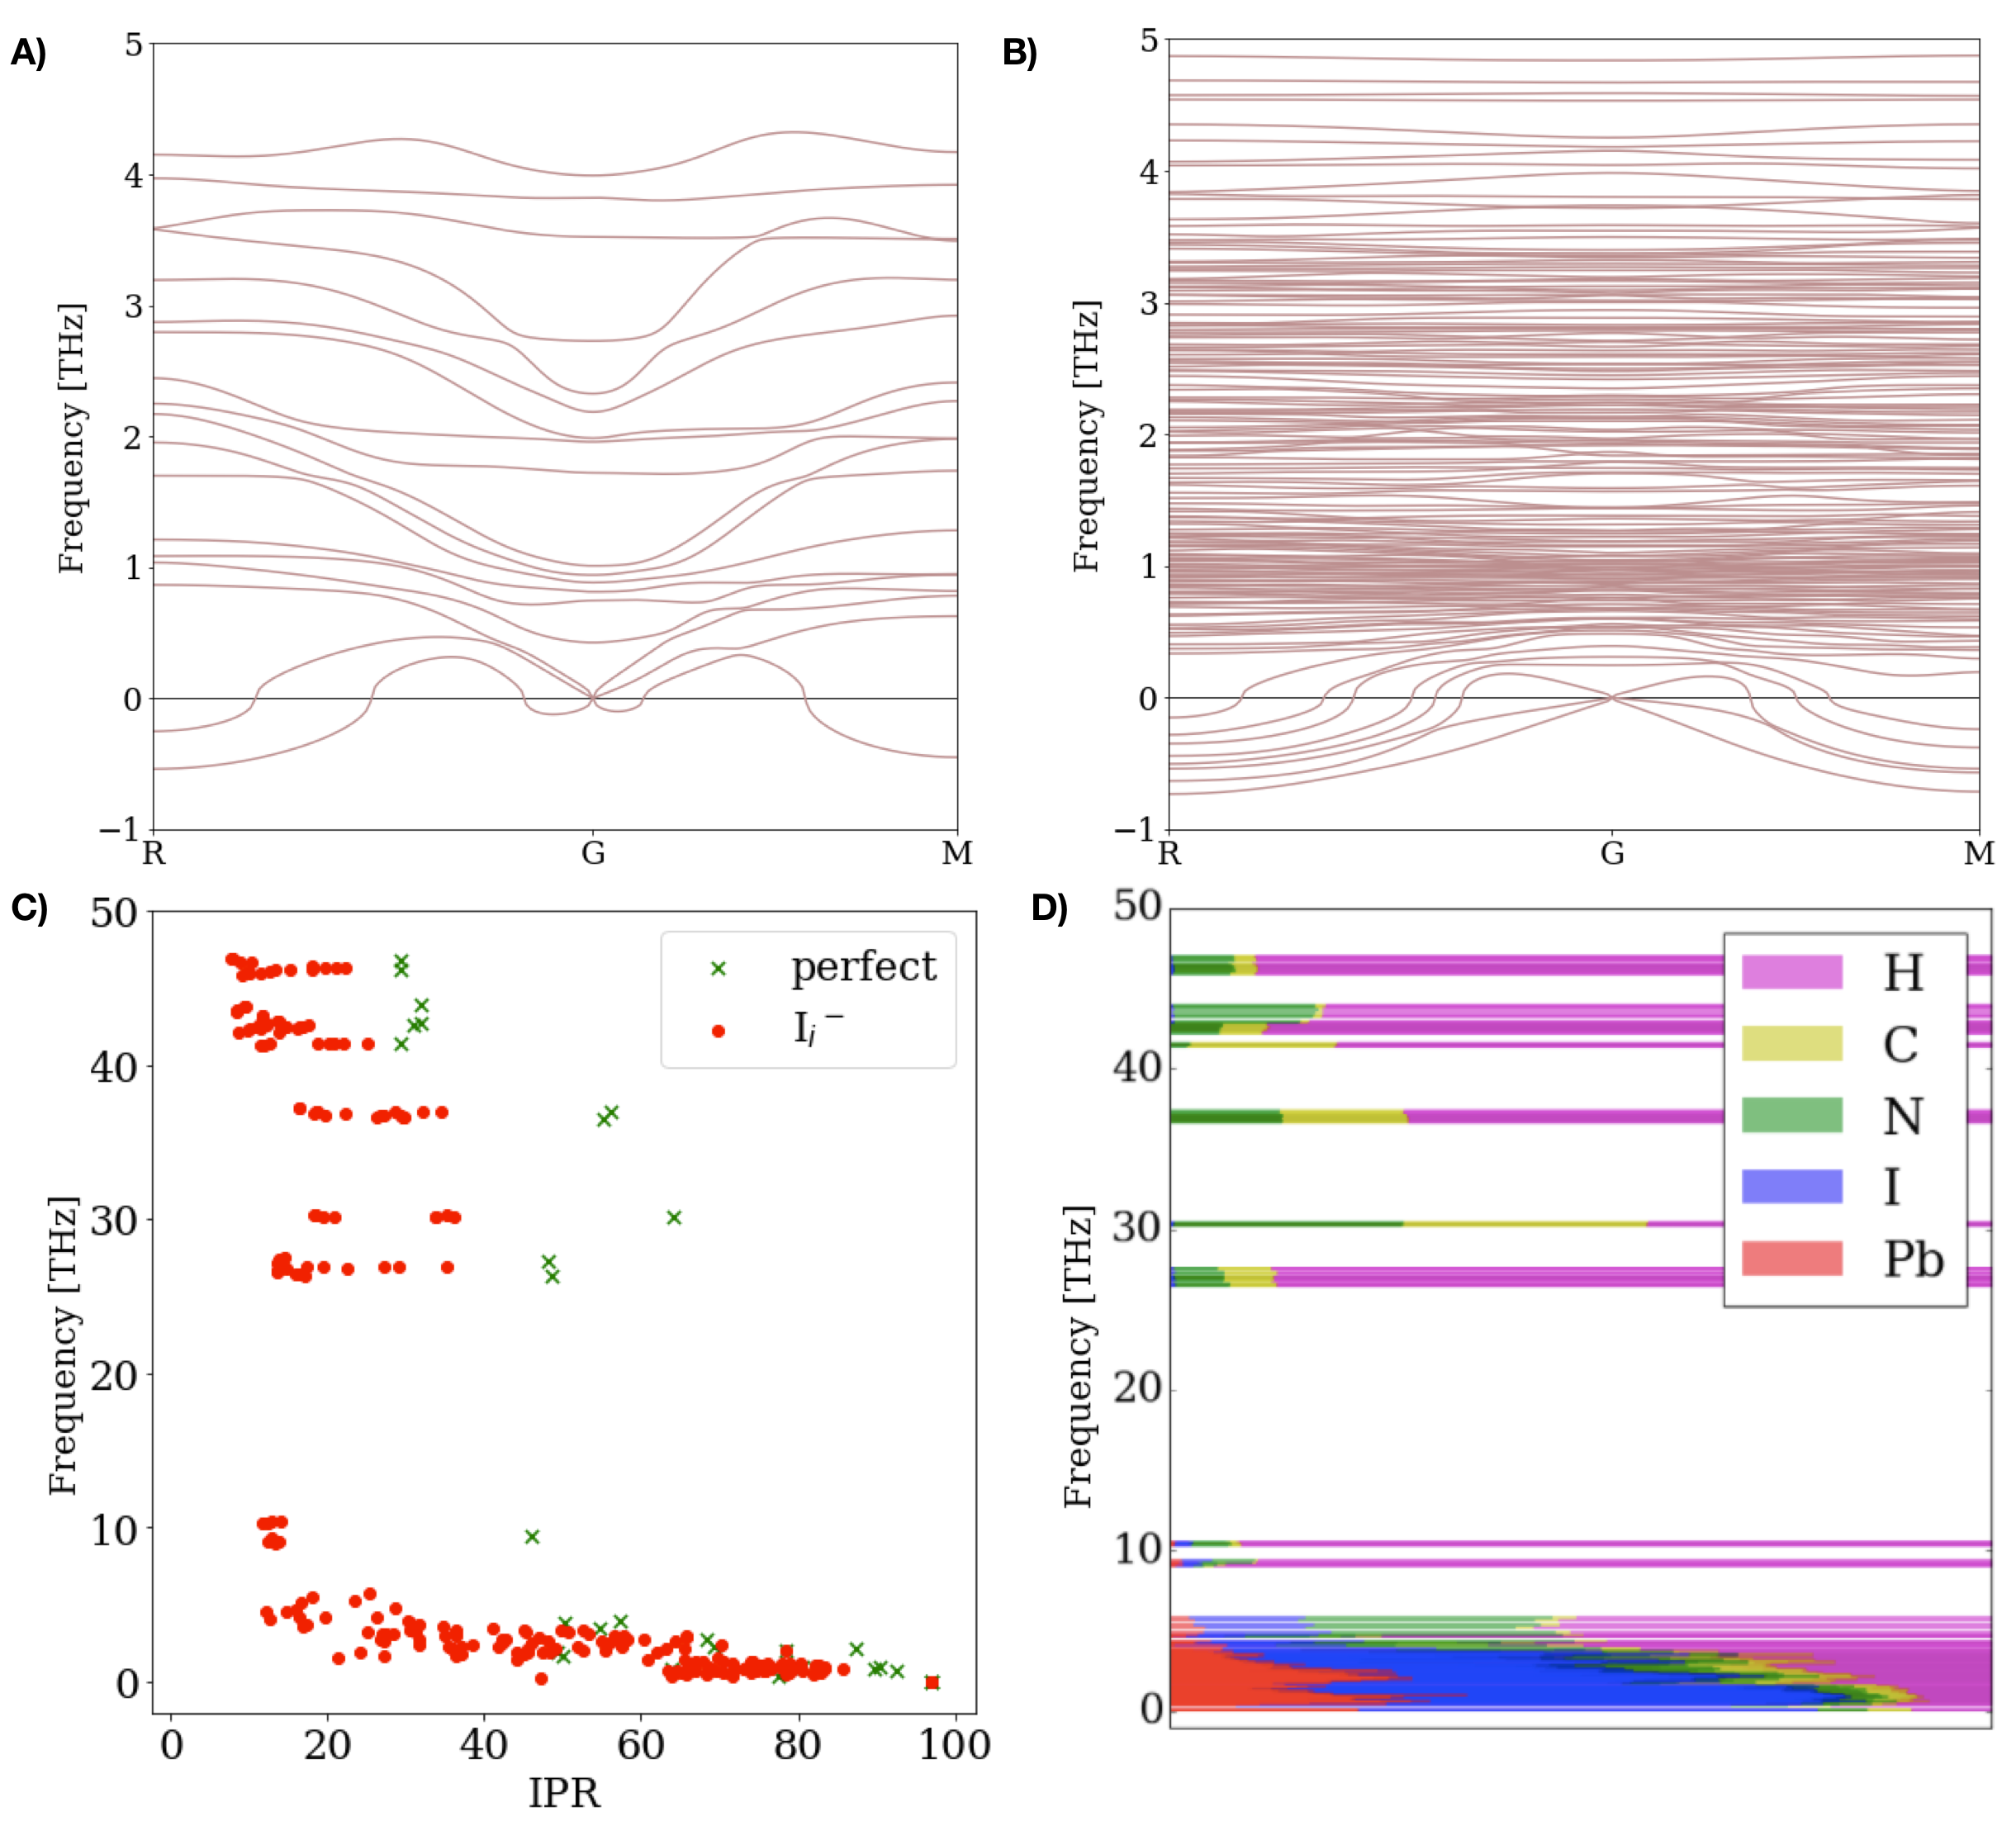
\includegraphics[width=1.0\columnwidth]{figures/ch6/defect_dispersion_IPR.png}
  \caption[Phonon dispersion and Inverse Participation Ratio of a MAPI crystal containing $\mathbf{I}_i^{-}$]{A) Harmonic phonon dispersion of the pristine lattice. The imaginary modes near the gamma point are the result of numerical noise from the sampling size of the fast fourier transform grid, and the imaginary modes at $R$ and $M$ correspond to the tilting of the inorganic octahedra. B) Harmonic phonon dispersion of a MAPI crystal containing $\mathrm{I}_i^{-}$} C) The Inverse Participation Ratio of a MAPI crystal containing $\mathrm{I}_i^{-}$} D) Contribution to phonon mode energy by atomic species.
\label{defect_dispersion_IPR}
\end{figure}

The complexity of the bandstructure makes it difficult to draw conclusions from a visual inspection of the phonon dispersion.
When translational invariance is lost, localised phonon states are introduced.
To identify which modes are associated with the iodine interstitial defect the inverse participation ratio can be used to quantify the localisation of phonon modes. 
The IPR is calculated from the harmonic phonon eigenvectors $e_i$ of the system. It is given by
\begin{equation}
\mathrm{IPR} = \frac{\left(\sum_{i=1}^N|e_i|\right)^2}{\sum_{i=1}^N\left(e_i|\right)^2},
\end{equation}
where N is the number of phonon modes. It gives a measure of how many atoms the phonon is distributed over. For example, for a chain of four atoms, a delocalised acoustic mode will have an $\textrm{IPR}=4$. At the other extreme, a phonon mode whose polarisation displaces only one atom will have an $\textrm{IPR}=1$.
The IPR of the gamma point phonon modes for the pristine and defective crystals are given in Figure \ref{defect_dispersion_IPR}c.
To allow for comparison, the IPR of the pristine lattice has been renormalised to give a maximum value of 97 for fully delocalised modes.
For both the perfect and defective lattice the IPR of the acoustic modes are equal to 97, so that they are completely delocalised, as is expected.
Figure \ref{defect_dispersion_IPR}c supports the conclusions drawn from the phonon dispersion; upon introduction of the defect each phonon mode of the pristine lattice `explodes' into multiple non-degenerate phonon modes of increased localisation.
Figure \ref{defect_dispersion_IPR}d splits the contribution to the phonon mode energy by element type. 
Lower energy phonon modes up to \SI{10{THz} include contributions from the I and Pb species, whilst the higher energy modes consist of vibrations from the light species associate with the \ce{CH3NH3PbI3}.

The contribution to the phonon mode energy can also be analysed by indidual atomic contributions.
The complete set of 291 phonon modes for the defective crystal is filtered to find that with the largest contribution from the two iodine interstitials associated with $\textrm{I}_2-$ defect bonding. This is a localised mode with an $\textrm{IPR}=21.4$ and a frequency of 1.59THz.
An animation of the phonon mode, generated using the ascii-phonons package,\autocite{} is available at \url{https://bit.ly/MAPI_phonon}.
This frequency is equal to the frequency of the harmonic potential energy surface of the negative iodine interstitial calculated in Section \ref{ch6:ccd}.
This is evidence that the single configuration coordinate $Q$ provides a good approximation to the accepting modes (modes that take up the electronic energy) of the charge transition.
As discussed in a paper by Alkauskas et al.,\autocite it may be surprising that a one-dimensional approximation to a multi-dimensional probem is sufficient, but this is particularly the case for defects with strong electron-phonon coupling.
We have shown in section \ref{ch5:ccd} that electron-phonon coupling is large, and the normal mode phonon calculations verify that the 1D configuration coordinate is a good approximation for the iodine interstitial defect in MAPI.




\subsection{Carrier capture coefficient} \label{finalsection}

In Section \ref{ch6:ccd} we used the extent of lattice relaxation on charge capture, $\Delta Q$, and the Huang-Rhys factor, $S$, as proxies to indicate the extent of electron phonon coupling. In this section we consider the electron phonon coupling matrix element (Equation \ref{epcouplingterm}) calculated from first principles and combine this with the solutions to the Schro\"{o}dinger for the anharmonic potential energy surfaces in Section \ref{ch6:cc} to calculate the electron capture coefficient at the neutral iodine interstitial. The electron capture coefficient $C_p$ determines the rate of electron capture $R_p$ via the following equation
\begin{equation}
R_p=C_pN_te
\end{equation}
%check that this consistent with earlier notation
where $N_t$ is the density of neutral defect traps and $e$ is the electron density.

During electron capture, a delocalised electron in the valence band is captured to a localised defect state. It is important that there is a single particle level in the bulk band gap for geometry $Q_0$ in Equation \ref{epcouplingterm}. There is an empty electronic defect state in the band gap at the equilibrium geometry for the neutral charge state (Figure \ref{eigenvalues}) and so this is chosen as $Q_0$.
\autocite{Alkauskas 2014}
In Figure \ref{eigenvalues} we see that as the lattice geometry is distorted towards that of the negative charge state the empty defect state decreases in energy until it is in the valence band and in the geometry of the negative charge state it is in the valence band and occupied by an electron. 
The change in overlap of the wavefunctions at the valence band minimum $\phi_i$ and unoccupied defect wavefunction $\phi_f$ gives a value of \SI{0.0036}{\electronvolt\per\amu\tothe{1/2}\per\angstrom} for the electron-phonon coupling matrix element.
It is possible to estimate the electron-phonon coupling term using an estimate of the degree of localisation of $\phi_i$ and $\phi_f$. For strong electron phonon coupling $W_if$ corresponds to 
\begin{equation}
W_{if} \approx \frac{\Delta E}{\Delta Q}\sqrt{\frac{M_d}{M_b}}
\end{equation}
where $M_b$ is the number of atoms in the supercell and $M_d$ is the number of atoms the defect state is localised on. $W_{if}\approx0.0037$ is obtained and so electron-phonon coupling for the single mode $Q$ is very strong.

\begin{figure}[h!]   
\centering
  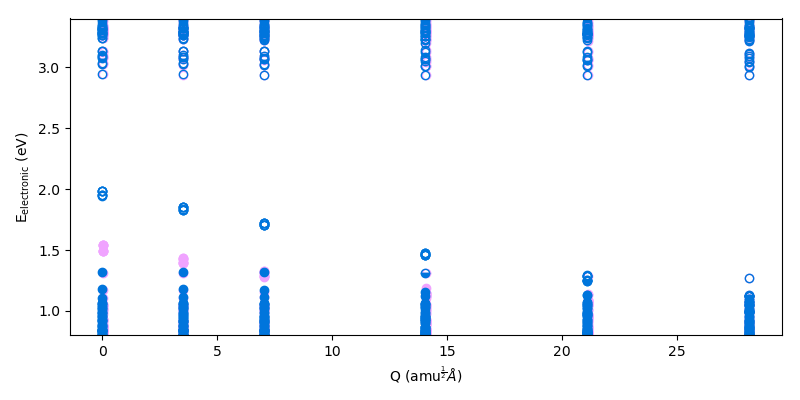
\includegraphics[width=1.0\columnwidth]{figures/ch6/eigs.png}
  \caption[ ]{}
\label{eigenvalues}
\end{figure}
%might need to label geometries

Combining the electron-phonon coupling term with solutions to the schrodinger equation for the neutral and negative charge state anharmonic potential energy surfaces as in Equation \ref{carriercapteqn}, the carrier capture coefficient at room temperature is \SI{1.2}{\centimetre\cubed\per\second}.
The large lattice distortion associated with charge capture suppresses radiative recombination, and the so non-radiative transition will be the dominant process.
\autocite{theory of defects in solids}


\begin{figure}[h!]   
\centering
  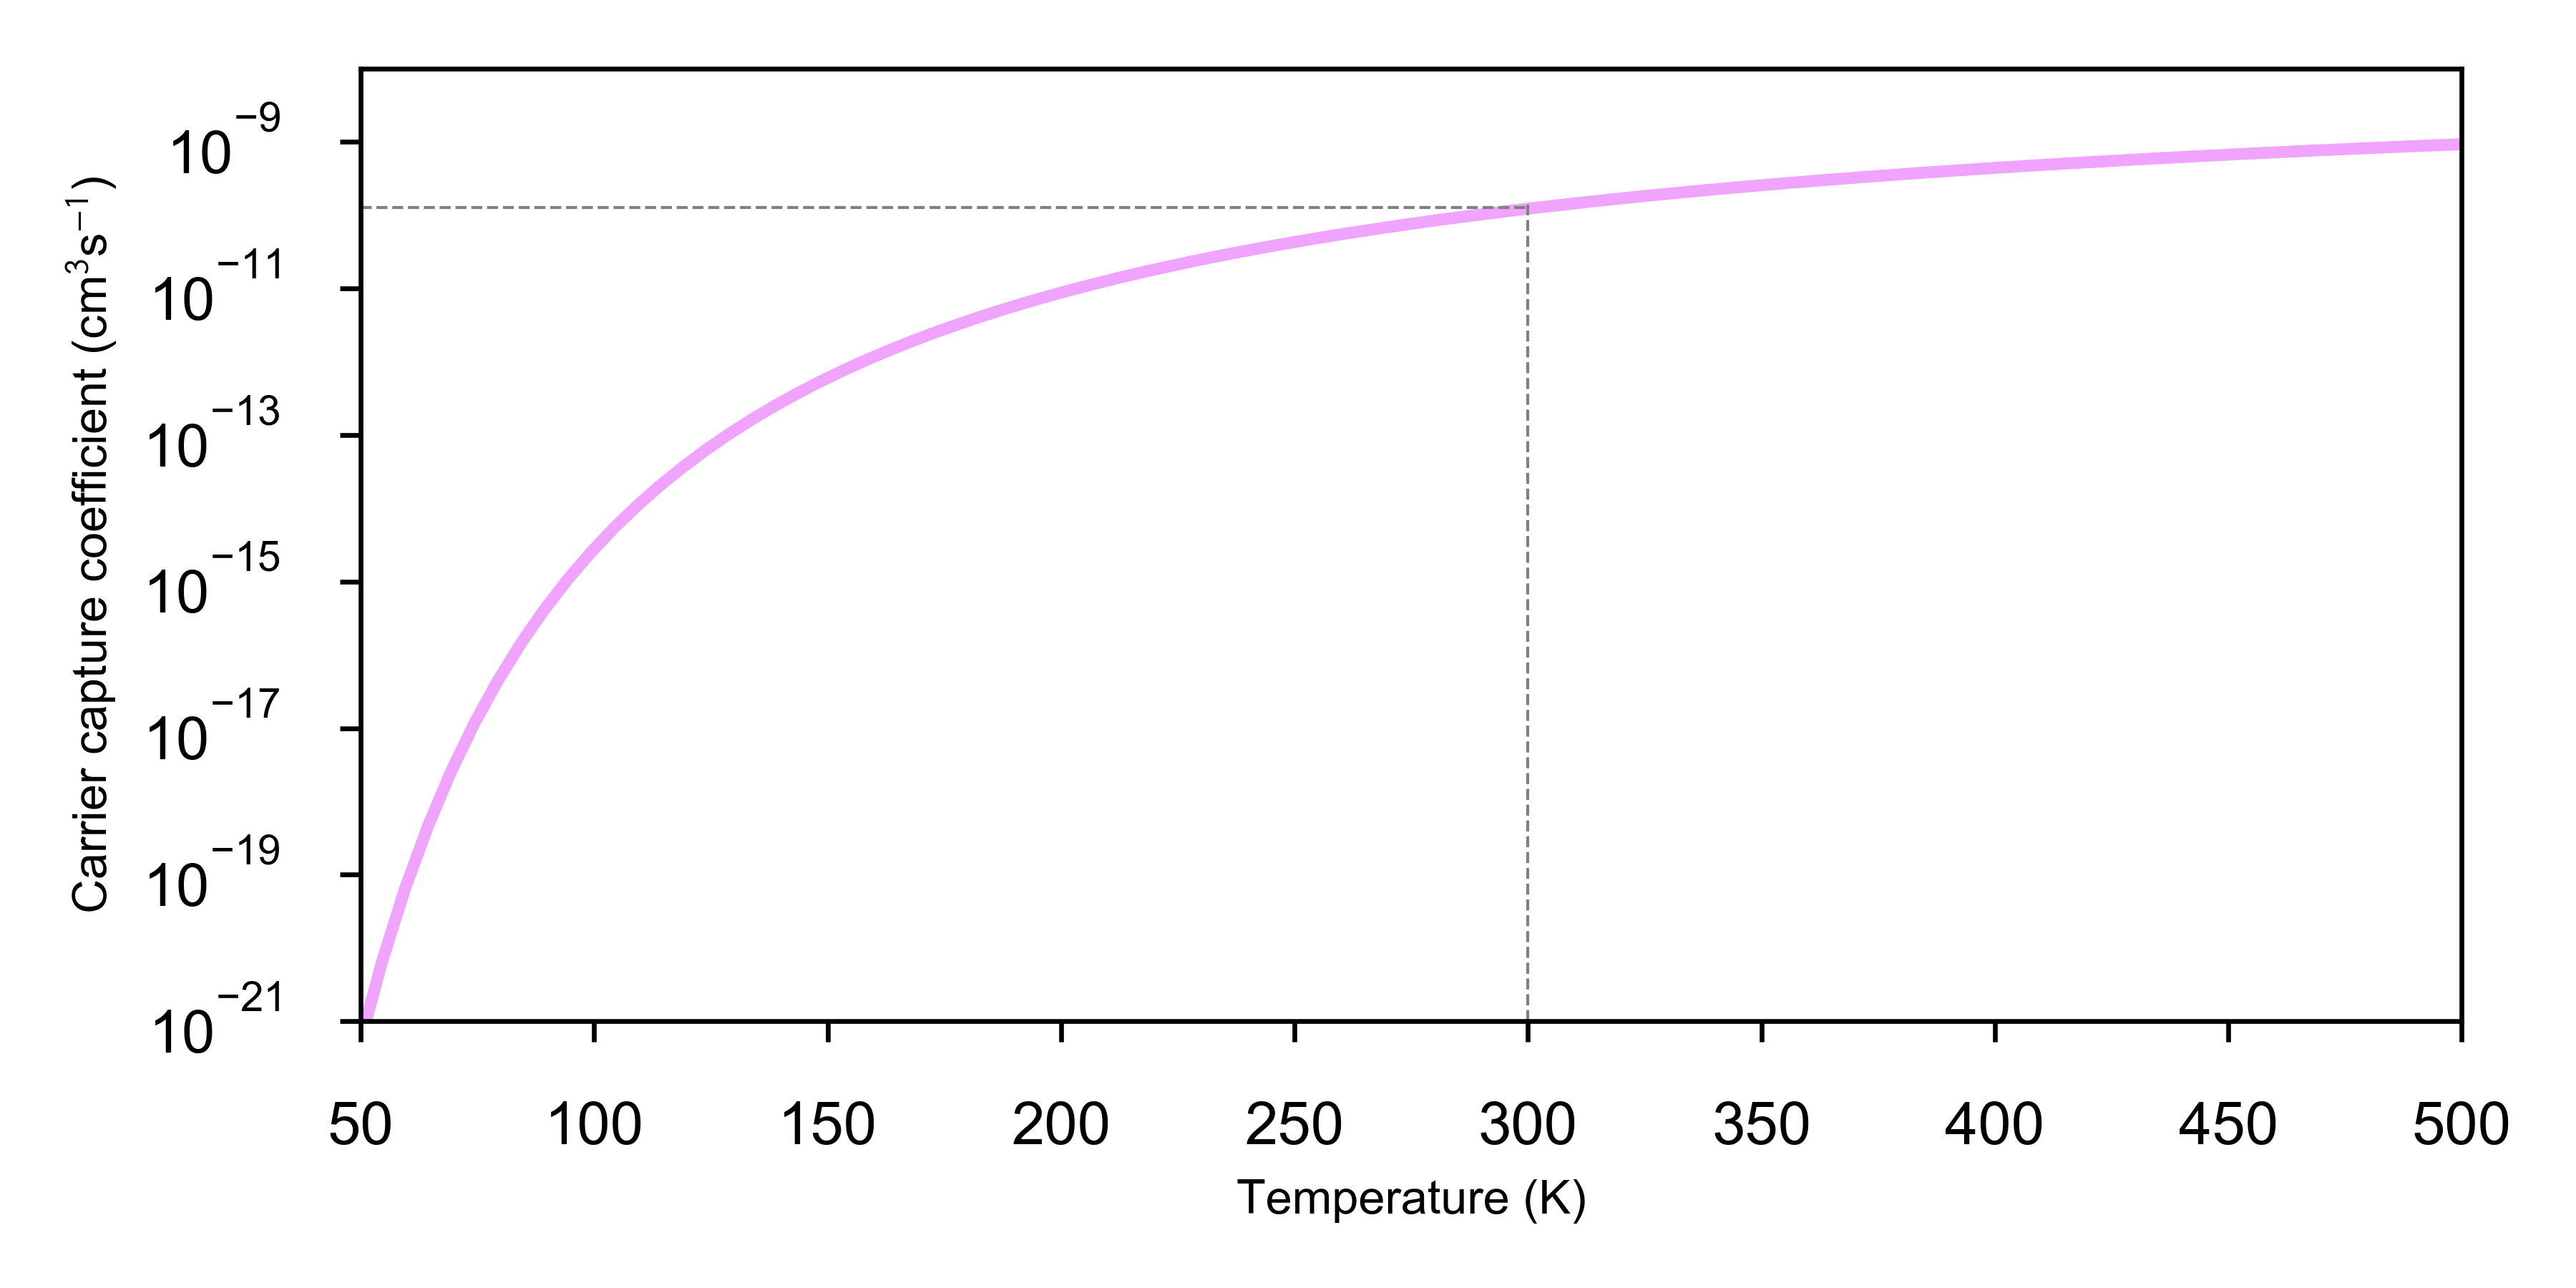
\includegraphics[width=1.0\columnwidth]{figures/ch6/carrier_capture_rate.png}
  \caption[Rate of electron capture at the ]{Configuration coordinate diagram for carrier capture between negative and neutral charge states of the iodine interstitial defect}
\label{carrier_capture_rate}
\end{figure}
%tabel of eigenstates like on Trello




\textbf{Summary}

The main conclusion of this study that electron capture at a neutral H-centre defect is fast, and that this process is a `one way street': due to the strong relaxation of the surrounding lattice, once a negative defect is formed it is both thermodynamically stable and stable under light irradiation.
The neutral defect is metastable and will be formed only after photo-excitation. The results demonstrate that the neutral defect cannot be formed from hole capture at a negative charge state, but the existing literature predicts that hole capture from the positive charge state is possible. Further calculations are needed to confirm this, and future work could apply the methodology developed here to this process. 

The results are consistent with the p-type doping observed in MAPI, which could be attributed to negatively charged interstitials, and the photo-induced `brightening'of perovskite photoluminsecence that is attributed to a reduction in trap state density.
%https://www.ncbi.nlm.nih.gov/pmc/articles/PMC6269531/#CR39
%https://www.nature.com/articles/ncomms11683
However we must be very careful in extrapolating to results beyond the bounds of this study,
as the model is limited in scope and the hybrid halide perovskites are complex materials. 
For example, it could be that there are other charge trapping mechanisms simultaneously occuring that involve longer polyiodide chains, lithium from the p-doped hole transporting material Spiro-OMETAD, or Au from the deposited electrodes. There are also open questions around charge trapping at the grain boundaries and surfaces.
%https://pubs.rsc.org/en/content/articlepdf/2019/cs/c8cs00853a

The results provide guidance for future studies of charge trapping in the hybrid halide perovskites.
We have shown that lattice anharmonicity is significant and that harmonic potential energy surfaces could lead to carrier capture coefficients that are many orders of magnitude too small (or large).
We have also found that the electron-phonon coupling term is large and this has two important consequences. Firstly, the relaxation of the whole lattice, not only the bonding atoms, must be considered in our calculations.
Secondly, for the electron capture process considered here, the single mode approximation is valid and the configuration coordinate $Q$ provides a good approximation to the accepting modes of negative iodine interstitial.

\textbf{Data access statement}

The crystal structures for the iodine interstitial in the negative, neutral and positive charge states reported in this chapter are available 
in an online repository.\autocite{}
The Inverse Participation Ratio (IPR) of the phonon modes can be calculated using the \textsc{JuliaPhonons} package available at.
The IPR data for the negative iodine interstitial, alongside the analysis steps taken to generate the results in this paper are available at \url{https://github.com/lucydot/MAPI_iodine_vibrations}
Carrier capture rates can be calculated using a package available at,%carriercapture
and the displacement between defect geometries can be visualised using .%vestavectors

\textbf{Acknowledgements}

Calculations were performed on the SiSu supercomputer at the IT Center for Science (CSC), Finland, via the Partnership for Advanced Computing in Europe (PRACE) project no. 13DECI0317/IsoSwitch.
Stoneham, Alkauskas, Subghyun Kim.
% Need to include TDDFT at start thesis